%%%%%%%%%%%%%%%%%%%%%%%%%%%%%%%%%%%%%%%%%%%%%%%%%%%%%%%%%%%%%%%%%
%%% %
%%% % weiiszablon.tex
%%% % The Faculty of Electrical and Computer Engineering
%%% % Rzeszow University Of Technology diploma thesis Template
%%% % Szablon pracy dyplomowej Wydziału Elektrotechniki 
%%% % i Informatyki PRz
%%% % June, 2015
%%%%%%%%%%%%%%%%%%%%%%%%%%%%%%%%%%%%%%%%%%%%%%%%%%%%%%%%%%%%%%%%%

\documentclass[12pt,twoside]{article}

\usepackage{weiiszablon}
\usepackage{hyperref}

\author{Mateusz Fesz}

% np. EF-123456, EN-654321, ...
\studentID{EF-167788}

\title{Implementacja wielowarstowej sieci neuronowej oraz algorytmu wstecznej propagacji błędu z adaptacyjnym współczynnikiem uczenia. Badanie wpływu metaparametrów sieci na efektywność uczenia}
\titleEN{Temat pracy po angielsku}


%%% wybierz rodzaj pracy wpisując jeden z poniższych numerów: ...
% 1 = inżynierska	% BSc
% 2 = magisterska	% MSc
% 3 = doktorska		% PhD
%%% na miejsce zera w linijce poniżej
\newcommand{\rodzajPracyNo}{0}


%%% promotor
\supervisor{(tytuł naukowy przed) Imię i nazwisko opiekuna (tytuł po)}
%% przykład: dr hab. inż. Józef Nowak, prof. PRz

%%% promotor ze stopniami naukowymi po angielsku
\supervisorEN{(academic degree) Imię i nazwisko opiekuna}

\abstract{Treść streszczenia po polsku}
\abstractEN{Treść streszczenia po angielsku}

\begin{document}

% strona tytułowa
\maketitle

\blankpage

% spis treści
\tableofcontents

\clearpage
\blankpage

\section{Opis projektu}
\subsection{Cel projektu}
Celem projektu jest realizacja uniwersalnej sieci neuronowej wielowarstwowej oraz zbadanie wpływu metaparametrów sieci na przebieg i efektywność procesu uczenia.
Metaparametry poddane badaniom to:
\begin{itemize}
	\item S1 - liczba neuronów w pierwszej warstwie sieci
	\item S2 - liczba neuronów w drugiej warstwie sieci
	\item lr - współczynnik uczenia sieci
	\item er - współczynnik maksymalnego dopuszczalnego przyrostu błędu, oznaczany również jako MAX\_PERF\_INC
	\item lr\textsubscript{dec} - modyfikator współczynnika uczenia w przypadku przekroczeniu maksymalnego dopuszczalnego przyrostu błędu
	\item lr\textsubscript{inc} - modyfikator współczynnika uczenia w przypadku spadku błędu
\end{itemize}

\subsection{Opis i przygotowanie wykorzystanych danych}
W celu przeprowadzenia badań, wykorzystany został zbiór danych dostępny pod adresem: \url{https://archive.ics.uci.edu/ml/datasets/zoo}.
Składa się na niego 101 rekordów opisanych 18 parametrami. Opisują one następujące cechy zwierzęcia:
\begin{enumerate}
	\item animal name - wartość tekstowa, stanowiąca nazwę zwierzęcia. Nieuwzględniana w procesie uczenia
	\item hair - wartość logiczna, określająca występowanie owłosienia na ciele zwierzęcia
	\item feathers, wartość logiczna, stwierdzająca występowanie piór na ciele zwierzęcia
	\item eggs - wartość logiczna, niosąca informację o składaniu przez zwierzę jaj
	\item milk - wartość logiczna, określająca zdolność zwierzęcia do wytwarzania mleka
	\item airborne - wartość logiczna, stwierdzająca zdolność zwierzęcia do lotu
	\item aquatic - wartość logiczna, niosąca informację o zdolności zwierzęcia do funkcjonowania w środowisku wodnym
	\item predator - wartość logiczna, informująca czy zwierzę jest drapieżnikiem
	\item toothed - wartość logiczna, określająca występowanie uzębienia u zwierzęcia
	\item backbone - wartość logiczna, stwierdzająca występowanie kręgosłupa
	\item breathes - wartość logiczna, niosąca informację o sposobie oddychania zwierzęcia
	\item venomous - wartość logiczna, określająca czy zwierzę jest jadowite
	\item fins - wartość loiczna, stwierdzająca występowanie płetw
	\item legs - wartość liczbowa, informująca o liczbie nóg danego zwierzęcia
	\item tail - wartość logiczna, niosąca informację o występowaniu ogona
	\item domestic - wartość logiczna, określająca czy zwierzę jest uznawane za domowe
	\item catsize - wartość logiczna, o niesprecyzowanej informacji
	\item type - wartość liczbowa, określająca przynależność zwierzęcia do jednej z siedmiu klas
\end{enumerate}

W procesie uczenia należy dokonać dopasowania zwierzęcia do odpowiedniej klasy.
Jako parametry przyjmuje się kolumny 2-17.
Kolumna 18 zawiera oczekiwaną wartość klasyfikacji.
Kolumna pierwsza nie jest wykorzystywana w procesie uczenia, gdyż nie opisuje ona fizycznej cechy zwierzęcia, a jedynie jego nazwę.

Przed przystąpieniem do procesu uczenia, przeprowadzono normalizację danych wejściowych. Wymagała jej jedynie kolumna ,,legs'' przyjmująca wartości numeryczne z zakresu $[0;8]$.
Numer klasy stanowiący jedyną daną wyjściową został natomiast przekształcony do postaci siedmio-elementowego wektora, zawierającego wartość $1$ na pozycji odpowiadającej danej klasie oraz wartości $0$ na pozostałych pozycjach.
W ostatnim kroku, dokonano podziału danych na zbiór uczący oraz zbiór walidacyjny.
W tym celu przydzielono $25\%$ rekordów należących do danej klasy do zbioru walidacyjnego, zaś pozostałą część do zbioru uczącego.

\section{Zagadnienia teoretyczne związane z wykorzystaną siecią neuronową oraz algorytmem uczenia}
\subsection{Model neuronu}
Neuron jest podstawowym elementem sieci neuronowej.
Jego elementami są:
\begin{itemize}
	\item Zbiór wejść $x$ długości $L$
	\item Zbiór powiązanych z wejściami wag $w$ długości $L$
	\item Wartość przesunięcia $b$
	\item Blok sumujący
	\item Funkcja aktywacji $f$
	\item Wyjście $a$
\end{itemize}


\begin{figure}[ht]
	\centering
	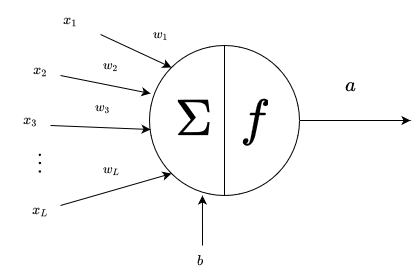
\includegraphics[width=12cm]{figures/models/neuronModel.png}
	\caption{Graficzny model neuronu}
	\label{Fig:neuron}
\end{figure}

Wartość sygnału wyściowego neuronu możemy określić wzorem:
\begin{equation}
	\label{eq:neuronOut}
	a = f\left(\sum\limits_{j=1}^{L}w_{j}x_{j} + b\right)
\end{equation}

W powyższym zapisie, $x_j$ oraz $w_j$ oznaczają odpowiednio kolejne wartości wejściowe i powiązane z nimi wagi (współczynniki wagowe).
Zapis ten możemy jednakże uprościć, zakładając że $x = \left[ x_1, x_2, ..., x_L\right]^T$ będzie wektorem kolumnowym wejść, $w = \left[ w_1, w_2, ..., w_L\right]$ - macierzą wierszową powiązanych z wejściami wag, natomiast wartości $a$ oraz $b$ - skalarami.
Wtedy równanie \ref{eq:neuronOut} przyjmie postać:
\begin{equation}
	\label{eq:neuronVec}
	a = f\left( w x + b \right)
\end{equation}

Ponadto istotnym w dalszych rozważaniach elementem modelu neuronu jest wyjście z bloku sumującego.
Oznaczając je jako $z$ otrzymamy:
\begin{equation}
	\label{eq:z}
	z = \sum\limits_{j=1}^{L}w_{j}x_{j} + b
\end{equation}

Obliczona w ten sposób wartość, stanowi argument funkcji aktywacji neuronu.
Funkcja ta przekształca wartość $z$ na inną wartość uzależnioną od jej charakterystyki.
Na potrzeby projektu, przyjęto że rolę tę będzie pełniła funkcja sigmoidalna (logsig).
Jej wartość możemy obliczyć zgodnie ze wzorem:
\begin{equation}
	\label{eq:sigmoid}
	f(z) =  \frac{1}{1 +\exp(-z)}
\end{equation}

W procesie uczenia istotna będzie także wartość pochodnej tej funkcji w danym punkcie.
W przypadku funkcji sigmoidalnej można ją sprowadzić do następującej postaci:
\begin{equation}
	\label{eq:sigmoidPrime}
	f'(z) = f(z) * 1-f(z)
\end{equation}
Co istotne, argumentami tej funkcji są stałe oraz wyliczona wcześniej pochodna w punkcie.
Właściwość ta może być użyta do zmniejszenia liczby wykonywanych przez algorytm operacji.


\subsection{Sieć neuronowa jednowarstwowa}
Siecią neuronową jednowarstwową nazywamy taką sieć, w której neurony nie są połączone ze sobą bezpośrednio, a jedynie otrzymują dane na wejściu i podają wynik na wyjście.

\begin{figure}[ht]
	\centering
	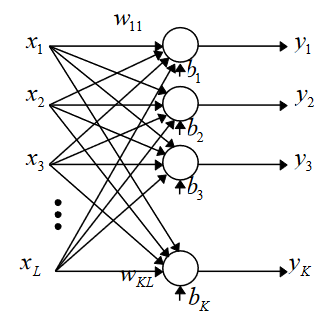
\includegraphics[width=12cm]{figures/models/singleLayerModel.png}
	\caption{Model prostej sieci jednowarstwowej}
	\label{Fig:singleNetwork}
\end{figure}

Wejściem każdego neuronu jest wektor sygnałów wejściowych $x$, zaś wyjściem sieci wektor $y = \left[ a_1, a_2, a_3, \cdots, a_K \right]^T$.
Ponadto możemy zdefiniować również wektor przesunięć $b = \left[ b_1, b_2, \cdots, b_K \right]$
Liczba wyjść z sieci jest tożsama z liczbą neuronów.

Wagi przyporządkowane wejściom można wyrazić w postaci macierzy o rozmiarach $K \times L$ gdzie $L$ oznacza liczbę wejść sieci, a $K$ liczbę neuronów.
$$\bm{w} = \left[
	\begin{array}{cccc}
		w_{11} & w_{12} & \cdots & w_{1L} \\
		w_{21} & w_{22} & \cdots & w_{2L} \\
		\vdots & \vdots &  & \vdots \\
		w_{K1} & w_{K2} & \cdots & w_{KL} \\
	\end{array}
	\right]$$

Przy założeniu że każdy neuron realizuje tą samą funkcję aktywacji, działanie sieci jednowartwowej wielowarstwowej możemy wyrazić w postaci macierzowej:
\begin{equation}
	\label{eq:singleLayerOut}
	a = f\left( wx + b \right)
\end{equation}
\subsection{Sieć neuronowa wielowarstwowa}
Siecią neuronową wielowarstwową, nazywamy taką sieć w której neurony ułożone są w dwóch lub więcej połączonych ze sobą warstwach.
Możemy zatem powiedzieć że jest to pewna liczba połączonych kaskadowo sieci jednowarstowych, a wyjście pojedynczej warstwy jest równocześnie wejściem warstwy następnej.
\begin{figure}[ht]
	\centering
	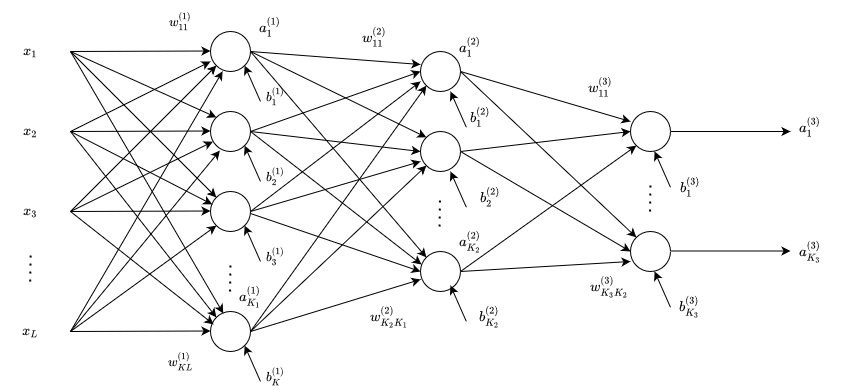
\includegraphics[width=14cm]{figures/models/manyLayerModel.png}
	\caption{Model prostej sieci trójwarstwowej}
	\label{Fig:multiNetwork}
\end{figure}

W przypadku tego typu sieci ilość macierzy wag jest równa liczbie warstw neuronów.
Oznaczając $a^{(l)}$ jako wyjście, $w^{(l)}$ jako macierz wag, $b^{(l)}$ jako macierz biasów, a $f^{(l)}$ jako funkcję aktywacji neuronów $l-$tej warstwy oraz wykorzystując równanie \ref{eq:singleLayerOut}, w przypadku sieci trójwarstwowej otrzymamy równania:
\begin{equation}
	\label{eq:tripleLayerOut}
	\begin{aligned}
		a^{(1)} &= f^{(1)} \left( w^{(1)} x + b^{(1)} \right)\\
		a^{(2)} &= f^{(2)} \left( w^{(2)} a^{(1)} + b^{(2)} \right)\\
		a^{(3)} &= f^{(3)} \left( w^{(3)} a^{(2)} + b^{(3)} \right)
	\end{aligned}
\end{equation}

Następnie, wykorzystując równania \ref{eq:tripleLayerOut}, możemy opisać działanie całej sieci trójwarstwowej równaniem:

\begin{equation}
	\label{eq:tripleLayerCombined}
	a^{(3)} &= f^{(3)} \left( w^{(3)} f^{(2)} \left( w^{(2)} f^{(1)} \left( w^{(1)} x + b^{(1)} \right) + b^{(2)} \right) + b^{(3)} \right)
\end{equation}

\subsection{Proces uczenia sieci z wykorzystaniem metody gradientowej}
Celem określenia sposobu uczenia sieci, koniecznym jest uprzednie zdefiniowanie tego, co oznacza określenie sieci ,,nauczoną'' bądź ,,nienauczoną''.
W tym celu definiujemy tzw. funkcję kosztu, określającą poziom rozbieżności pomiędzy wartością otrzymaną na wyjściu sieci, a wartością oczekiwaną.
Przykładem takiej funkcji, jest funkcja błędu średniokwadratowego (MSE):
\begin{equation}
	\label{eq:costFunction}
	C\left( w, b, x, a\right) = \frac{1}{2n} \sum\limits_{x} || y\left( x \right) - a ||^2
\end{equation}

W powyższym równaniu, $w$ określa zbiór wszystkich wag wewnątrz sieci, $b$ wszystkich jej biasów, $x$ zbiór danych wejściowych, $n$ ilość danych wejściowych, $y(x)$ zbiór oczekiwanych danych wyjściowych, natomiast $a$ zbiór uzyskanych wyjść z sieci.
Zakładając, że w procesie uczenia wartości $x$ oraz $a$ pozostają stałe, możemy uprościć oznaczenie funkcji do postaci $C (w,b)$.
Funkcja ta dąży do 0 gdy wartości otrzymywane na wyjściu sieci są bliskie wartościom oczekiwanym, i rośnie wraz ze wzrostem różnicy pomiędzy nimi.
W związku z powyższym, należy znaleźć taką metodę, która pozwoli na minimalizację wartości funkcji $C(w,b)$.

\subsubsection{Ogólny algorytm gradientowy}
Celem zobrazowania problemu rozważmy prostą funkcję $C(v_1, v_2)$ zobrazowaną na rysunku \ref{Fig:simpleCost}.
Naszym celem jest znalezienie jej globalnego minimum.
Teoretycznie możliwe jest jego wyznaczenie metodą analityczną, jednakże według literatury \cite{nndl} jest to rozwiązanie mało wydajne, szczególnie gdy rozważymy funkcje więcej niż kilku zmiennych.

\begin{figure}[ht]
	\centering
	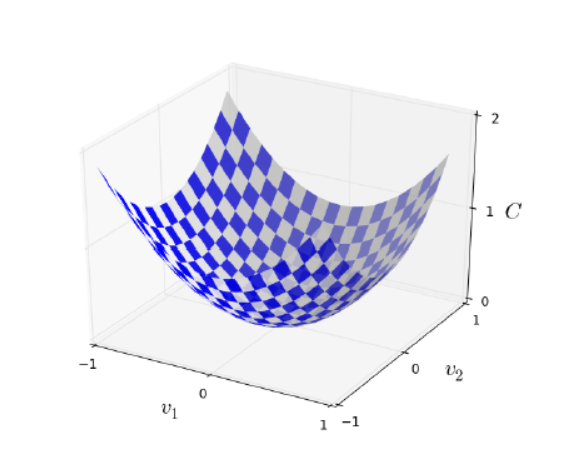
\includegraphics[width=12cm]{figures/models/gradientExample.png}
	\caption{Przykładowa funkcja 2 zmiennych}
	\label{Fig:simpleCost}
\end{figure}

Obserwując rysunek \ref{Fig:simpleCost} możemy jednak dojść do znacznie prostszej obliczeniowo metody.
Przyjmując bliskie zeru wartości $\Delta v_1$ oraz $\Delta v_2$ możemy przyjąć zmianę wartości funkcji $C(v_1, v_2)$ na poziomie:
\begin{equation}
	\label{eq:deltaC}
	\Delta C \approx \frac{\delta C}{\delta v_1} \Delta v_1 + \frac{\delta C}{\delta v_2} \Delta v_2
\end{equation}

Na podstawie powyższego równania możemy zdefiniować wektor zmian:
\begin{equation}
	\label{eq:changeVector}
	\Delta v = (\Delta v_1, \Delta v_2)^T
\end{equation}
oraz tzw. wektor gradientu:
\begin{equation}
	\label{eq:gradientVector}
	\nabla C = \left(\frac{\delta C}{\delta v_1},\frac{\delta C}{\delta v_1}\right)^T
\end{equation}

Wykorzystując powyższe definicje, równanie \ref{eq:gradientVector} możemy zapisać w postaci:
\begin{equation}
	\label{eq:costGradientVector}
	\Delta C \approx \nabla C \cdot \Delta v
\end{equation}

Problemem przy równaniu \ref{eq:costGradientVector} jest wyznaczenie optymalnego wektora $\Delta v$, tak aby zagwarantować ujemną wartość $\Delta C$. W tym celu, możemy przyjąć wartości opisywane równaniem \ref{eq:changeVector} jako równe:
\begin{equation}
	\label{eq:lrNabla}
	\Delta v = -\eta \nabla C
\end{equation}

Wartość $\eta$ nazywana jest ,,współczynnikiem uczenia'' i przyjmuje bliskie zeru, dodatnie wartości. Wykorzystując powyższą definicję, możemy zapisać równanie \ref{eq:costGradientVector} w postaci:
\begin{equation*}
	\begin{aligned}
		\Delta C &\approx - \eta \nabla C \cdot \nabla C\\
		\Delta C &\approx - \eta ||\nabla C||^2
	\end{aligned}
\end{equation*}
W tej postaci równania widzimy, że dla odpowiednio niskiego współczynnika $\eta$ zagwarantowany jest spadek wartości funkcji kosztu $C(v)$.
Wykorzystując właściwość opisaną równaniem \ref{eq:lrNabla} możemy wyznaczyć nowe wartości zmiennych zawartych w wektorze $v$:
\begin{equation}
	\begin{aligned}
		v  \rightarrow v' &= v - \eta \nabla C \\
		v' &= v + \Delta v
	\end{aligned}
\end{equation}

Wielokrotnie aplikując powyższą regułę, jesteśmy w stanie podążać za gradientem aż do osiągnięcia minimum.
Literatura \cite{nndl} definiuje ją jako ,,algorytm spadku gradient'', ale jednocześnie wspomina że w niektórych sytuacjach, może nie być w pełni skuteczna.

\subsubsection{Zastosowanie algorytmu gradientowego w sieciach wielowarstwowych}

Algorytm gradientowy może zostać wykorzystany do minimalizacji funkcji przedstawionej równaniem \ref{eq:deltaC}, poprzez odnajdowanie wartości wag oraz biasów minimalizujących funkcję kosztu.
Wykorzystując oznaczenia $w^{(l)}_{ij}$ jako j-tą wagę i-tego neuronu l-tej warstwy oraz $b^{(l)}_i$ jako bias i-tego neuronu w l-tej warstwie, możemy wyznaczyć ich wartości w kolejnych iteracjach (epokach) procesu uczenia:
\begin{equation}
	\label{eq:weightUpdate}
	w^{(l)}_{ij} \rightarrow {w'}^{(l)}_{ij} = w^{(l)}_{ij} - \eta \frac{\delta C}{\delta w^{(l)}_{ij}}
\end{equation}
\begin{equation}
	\label{eq:biasUpdate}
	b^{(l)}_{i} \rightarrow {b'}^{(l)}_{i} = b^{(l)}_{i} - \eta \frac{\delta C}{\delta b^{(l)}_{i}}
\end{equation}

Przyjmując jako funkcję kosztu błąd średniokwadratowy, przy założeniu wystąpienia wielu danych uczących, możemy ją zapisać w postaci:
\begin{equation}
	C = \frac{1}{n} \sum \limits_x C_x
\end{equation}
czyli średniej wartości błędów $C_{x} = \frac{||y(x) - a||^2}{2}$ dla poszczególnych par uczących.

TODO: Rozpisać wzory na poszczególne pochodne - instrukcja \cite{kiaMultiLayer}



\subsubsection{Metoda stochastycznego spadku gradientu}
Jednym z problemów algorytmu spadku gradientu, objawiającym się przy dużej liczbie rekordów uczących \cite{nndl} jest długi czas potrzebny na obliczanie wartości pochodnych w równaniu \ref{eq:gradientVector}.
Celem zniwelowania tego problemu można wykorzystać metodę zwaną ,,stochastycznym spadkiem gradientu''.
Polega ona na oszacowaniu rzeczywistego gradientu $\nabla C$ poprzez obliczenie $\nabla C_x$ dla losowo wybranej próbki danych uczących.
Poprzez odpowiednie dobranie rozmiaru próbek, oraz ich odpowiednie uśrednienie, możemy uzyskać dobre przybliżenie rzeczywistego gradientu $\nabla C$.\cite{nndl}
Elementy pojedynczej próbki możemy oznaczyć jako $X_1, X_2, \ldots , X_m$
Zakładając odpowiednio duży rozmiar $m$ możemy przyjąć za prawdziwe równanie:
\begin{equation}
	\label{eq:stochasticGradient}
	\frac{ \sum_{j=1}^{m} \nabla C_{X_j}}{m} \approx \frac{ \sum_x \nabla C_x}{n} = \nabla C
\end{equation}

Przenosząc czynnik $\frac{1}{m}$ przed znak sumy, otrzymamy:
\begin{equation}
	\label{eq:stochasticGradientFinal}
	\nabla C \approx \frac{1}{m} \sum_{j=1}^{m} \nabla C_{X_j}
\end{equation}

Wartym zauważenia jest też fakt występowania różnych konwencji uśredniania czy też skalowania gradientu stochastycznego. \cite{nndl}
Niektóre źródła mówią o braku konieczności ich stosowania gdyż wpływają na działanie sieci jedynie pośrednio, poprzez modyfikację wartości współczynnika uczenia.
Z tego też powodu, w dalszej implementacji przyjęto współczynnik równy stosunkowi rozmiaru próbki do rozmiaru całego zbioru uczącego.

\subsubsection{Adaptacyjny współczynnik uczenia}
W równaniu \ref{eq:lrNabla} wprowadzono pojęcie współczynnika uczenia.
Standardowa metoda gradientowa zakłada że jest on stały przez cały okres uczenia sieci, a jego odpowiedni dobór jest jednym z kryteriów koniecznych do poprawnego przebiegu procesu uczenia.
Nie jest to jednak rozwiązanie optymalne, gdyż zbyt duża jego wartość może znacząco utrudnić osiągnięcie minimum funkcji błędu a w skrajnych przypadkach spowodować rozbiegnięcie procesu uczenia.
Zbyt mała jego wartość również jest niekorzystna gdyż znacznie wydłuża czas potrzebny na osiągnięcie celu uczenia - definiowanego jako minimalizacja funkcji wyrażonej równaniem \ref{eq:costFunction}.

Jedną z metod pozwalających zniwelować ten problem, jest metoda adaptacyjnej korekty współczynnika uczenia $\eta $\cite{kiaAcc}.
Przyjmując wartość błędu w chwili czasu $t$:
\begin{equation}
	\label{eq:costFunctionTimed}
	MSE(t) = \frac{1}{2n} \sum_{i=1}^{M}  || y_{i}(t) - a(t) ||^2
\end{equation}
Możemy zdefiniować sposób korekty współczynnika uczenia jako:
\begin{equation}
	\label{eq:adaptiveLR}
	\eta \left( t + 1 \right)  =
	\begin{cases}
		\eta \left( t \right) \cdot \xi_d & \text{gdy } MSE(t) > er \cdot MSE(t-1)\\
		\eta \left( t \right) \cdot \xi_i & \text{gdy } MSE(t) <  MSE(t-1)\\
		\eta \left( t \right)  & \text{gdy } MSE(t-1) \leq MSE(t) \leq er \cdot MSE(t-1)
	\end{cases}
\end{equation}
gdzie $\xi_d$ $\xi_i$ są odpowiednio współczynnikami zmniejszania i zwiększania wartości współczynnika uczenia, zaś $er$ określa dopuszczalną krotność przyrostu błędu.
Podejście takie powoduje wprawdzie konieczność ustalenia dodatkowych parametrów w procesie uczenia, lecz eliminuje problem doboru współczynnika uczenia.
Jeśli będzie on zbyt duży, zostanie zredukowany do pożądanego poziomu ze względu na wzrastający poziom błedu.
Jednocześnie zbyt niska wartość $\eta$ zostanie zwiększona kiedy proces uczenia natrafi na bardziej optymalne warunki.

Literatura \cite{nnd} podaje także bardziej skomplikowany wariant zastosowania zmiennego współczynnika uczenia.
Polega on na dodatkowym zapisywaniu stanu wag oraz biasów przed ich zmianą wynikającą z algorymtu spadku gradientu.
Wagi te mogą następnie zostać przywrócone jeśli uczenie przyniosło efekt odwrotny do zamierzonego i doszło do wzrostu wartości błędu.
W praktyce oznacza to przywrócenie zachowanych wag oraz biasów w momencie zmniejszenia $\eta$ o współczynnik \xi_d.

\section{Implementacja algorytmów w języku Rust}
Przed wykonaniem badań operujących na przedstawionych algorytmach, konieczna była ich implementacja w postaci pozwalającej na proste ustalanie parametrów sieci, oraz jej ewentualne modyfikacje na potrzeby eksperymentów.
W tym celu wykorzystany został język programowania ogólnego przeznaczenia - Rust, oraz następujące biblioteki:
\begin{itemize}
	\item ndarray 0.15.4 - wykorzystywana do obliczeń związanych z algebrą liniową, przede wszystkim operacji na macierzach
	\item rand 0.8.5 - wykorzystywana do generowania liczb losowych
\end{itemize}
Pełny kod gotowy do kompilacji i uruchomienia znajduje się na repozytorium: \url{https://github.com/MatiF100/AI_Project}.

\subsection{Implementacja struktury sieci}
\subsubsection{Podstawowa struktura reprezentująca sieć}
Pierwszym krokiem koniecznym do realizacji projektu było wykonanie ogólnej struktury sieci, pozwalającej na ustalenie jej parametrów, oraz funkcji pozwalającej na jej inicjalizację.


\begin{lstlisting}[language=Rust,caption=Podstawowa struktura sieci neuronowej,label={lst:netStructure}]
#[derive(Debug, Clone)]
struct Network {
    layers: Vec<usize>,
    biases: Vec<Array2<f64>>,
    weights: Vec<Array2<f64>>,
    name: String,
}
\end{lstlisting}

\begin{lstlisting}[language=Rust,caption=Konstruktor struktury sieci neuronowej,label={lst:netConstructor}]
fn new(layers: Vec<usize>) -> Self {
	let mut rng = rand::thread_rng();
	let layers = layers
		.into_iter()
		.filter(|x| *x > 0)
		.collect::<Vec<usize>>();
	Self {
		name: String::from("Network 0"),
		//Biases are initialized with random values
		biases: layers
			.iter()
			.skip(1)
			.map(|&s| {
				(0..s)
					.map(|_| rng.gen_range::<f64, std::ops::Range<f64>>(-1.0..1.0))
					.collect::<Vec<f64>>()
			})
			.map(|v| Array2::from_shape_vec((v.len(), 1), v).unwrap())
			.collect(),

		//Weights are also initialized with random values
		weights: layers
			.windows(2)
			.map(|x| {
				(
					(x[0], x[1]),
					(0..x[0] * x[1])
						.map(|_| rng.gen_range::<f64, std::ops::Range<f64>>(-1.0..1.0))
						.collect::<Vec<f64>>(),
				)
			})
			.map(|(x, v)| Array2::from_shape_vec((x.1, x.0), v).unwrap())
			.collect::<Vec<_>>(),
		//Layers are moved in from the argument
		layers,
	}
}

\end{lstlisting}

Sieć została zbudowana w sposób dający dużą swobodę w ustalaniu jej parametrów - zarówno liczba warstw jak i neuronów w poszczególnych warstwach może być łatwo modyfikowana przez podanie odpowiedniego wektora jako argumentu.


\begin{lstlisting}[language=Rust,caption=Utworzenie przykładowej struktury sieci,label={lst:netExample}]
fn main(){
	let (R, S1, S2, S3) = (16, 8, 6, 2);
	let x = Network::new(vec![R, S1, S2, S3]);
}
\end{lstlisting}

Powyższy kod tworzy sieć neuronową o 16 wejściach, 8 neuronach w warstwie 1, 6 neuronach w warstwie drugiej oraz 2 neuronach w warstwie trzeciej.
Dla uproszczenia kodu i przyspieszenia obliczeń, wejścia sieci są reprezentowane jako dodatkowa warstwa neuronów, których wyjście w trakcie działania sieci jest ustalane do wartości znajdujących się w wektorze wejściowym.
Również dla uproszczenia kodu, przyjęto stałą funkcję aktywacji dla każdego z neuronów, opisaną równaniem \ref{eq:sigmoid}.


\begin{lstlisting}[language=Rust,caption=Funkcja sigmoidalna oraz jej pochodna,label={lst:sigmoid}]
//Sigmoidal function - basic activation function for neurons
fn sigmoid<D>(z: Array<f64, D>) -> Array<f64, D>
where
    D: Dimension,
{
    let mut z = z;
    z.iter_mut().for_each(|f| *f = 1.0 / (1.0 + (-*f).exp()));
    z
}

//Derivative of sigmoidal function
fn sigmoid_prime<D>(z: Array<f64, D>) -> Array<f64, D>
where
    D: Dimension,
{
    let val = sigmoid(z);
    &val * (1.0 - &val)
}
\end{lstlisting}

Powyższa implementacja nie jest optymalna, gdyż zakłada obliczanie wartości funkcji aktywacji przy każdym wywołaniu funkcji zwracającej jej pochodną, podczas gdy zwykle wartość ta była już obliczona wcześniej.
Możliwe jest zatem dalsza optymalizacja kodu, co jednakże nie jest konieczne dla przeprowadzenia większości eksperymentów.


\begin{lstlisting}[language=Rust,caption=Realizacja funkcji feed-forward,label={lst:feedforward}]
fn feed_forward(&self, mut a: Array2<f64>) -> Array2<f64> {
	for (b, w) in self.biases.iter().zip(self.weights.iter()) {
		a = sigmoid(w.dot(&a) + b);
	}
	return a;
}
\end{lstlisting}

Ostatnią funkcją konieczną do działania sieci jest funkcja feedforward, pobierająca dane z wejścia sieci, i zwracająca wynikowy wektor stopnia aktywacji neuronów wyjściowych.

\subsubsection{Algorytm uczenia sieci}
\begin{lstlisting}[language=Rust,caption=Realizacja funkcji stochastycznego spadku gradientu,label={lst:sgd}]
 fn sgd(
	&mut self,
	training_data: &mut Vec<(Array2<f64>, Array2<f64>)>,
	epochs: usize,
	mini_batch_size: usize,
	mut eta: f64,
	test_data: Option<&Vec<(Array2<f64>, usize)>>,
	eta_mod: Option<(f64, f64)>,
	target_cost: f64,
	report_interval: usize,
) {
	let mut rng = rand::thread_rng();

	//Main loop performing learning step with each epoch
	for j in 1..=epochs {
		//Randomization of data for usage of mini-batch
		training_data.shuffle(&mut rng);

		//Generation of mini-batch vector. This is basicaly a collection of smaller datasets
		let mut mini_batches = training_data
			.windows(mini_batch_size)
			.step_by(mini_batch_size)
			.map(|s| s.to_vec())
			.collect::<Vec<Vec<_>>>();

		let batch_count = mini_batches.len();
		// Branching based on existance of adaptive learning rate parameters
		match eta_mod {
			Some((dec, inc)) => {
				// Saving state of network before readjustment of weights and biases
				let saved_weights = self.weights.clone();
				let saved_biases = self.biases.clone();
				let previous_error = self.mse(training_data);

				//Sub-loob performing learning step for each of the mini-batch
				for mini_batch in &mut mini_batches {
					//dbg!(&mini_batch);
					self.update_mini_batch(mini_batch, eta, batch_count)
				}

				// Verification of newly achieved Mean Square Error
				let new_error = self.mse(training_data);
				if new_error < target_cost {
					if let Some(data) = &test_data {
						let output = self.evaluate(data);
						println!("{},{}", self.name, output.1 as f64 / output.0 as f64);
					}
					break;
				}
				if new_error > previous_error * MAX_PERF_INC {
					// Restoring backup
					self.weights = saved_weights;
					self.biases = saved_biases;

					// Adaptation - learning rate decreases
					eta *= dec;
				} else if new_error < previous_error {
					// Adaptation - learning rate increases
					eta *= inc;
				}
				// else statement does nothing - ommited
			}
			None => {
				//Sub-loob performing learning step for each of the mini-batch
				for mini_batch in &mut mini_batches {
					//dbg!(&mini_batch);
					self.update_mini_batch(mini_batch, eta, batch_count);
					let new_error = self.mse(training_data);
					if new_error < target_cost {
						if let Some(data) = &test_data {
							let output = self.evaluate(data);
							println!("{},{}", self.name, output.1 as f64 / output.0 as f64);
						}
						break;
					}
				}
			}
		}

		//Data verification. Can be ommited
		if let Some(data) = &test_data {
			if j + 1 % report_interval == 0 && report_interval != 0 {
				let output = self.evaluate(data);
				println!("{},{}", self.name, output.1 as f64 / output.0 as f64);
			}
		} else {
			//println!("Epoch {} complete!", j);
		}
	}
}
\end{lstlisting}

Powyższy kod realizuje uogólniony przypadek funkcji spadku gradientu.
W jego ramach można wyróżnić kilka bloków funkcjonalnych.
Pierwszym z nich jest definicja funkcji spadku gradientu oraz jej parametrów:
\begin{itemize}
	\item &mut self - mutowalna referencja do struktury Network, słowo kluczowe self oznacza że funkcja stanowi metodę struktury Network
	\item training\_data - mutowalna referencja do wektora przechowującego pary uczące
	\item epochs - maksymalna liczba epok przez które należy wykonywać algorytm
	\item mini\_batch\_size - rozmiar próbki w metodzie stochastycznej (ustawiona na wartość równą długości wektora training\_data będzie równoważne z brakiem podziału danych uczących)
	\item mut eta - mutowalna wartość zmiennoprzecinkowa, współczynnik uczenia
	\item test\_data - opcjonalna referencja do wektora przechowującego dane wykorzystywane do walidacji krzyżowej
	\item eta\_mod - opcjonalne parametry wykorzystywane w ramach adaptacyjnego współczynnika uczenia
	\item target\_cost - docelowy błąd
	\item report\_interval - liczba epok co którą sieć wykonuje walidację krzyżową i wyświetla raport
\end{itemize}

Następnym etapem, działającym już wewnątrz pętli jest wykonanie  podziału zbioru uczącego na mniejsze próbki (o ile następuje taka konieczność).
Dalsza część funkcji opiera się na opcjonalnym parametrze eta\_mod.
Jeśli jest on obecny, wykonywany jest algorytm powiązany z adaptacyjnym współczynnikiem uczenia.
W każdej iteracji pętli, parametry sieci oraz poprzedni błąd są zapisywane przed wykonaniem operacji uczenia, a następnie w zależności od uzyskanego wyniku, wykonywana jest jedna z operacji opisana w równaniu \ref{eq:adaptiveLR}.
Jeżeli natomiast nie podano parametrów modyfikacji współczynnika uczenia, wykonywany jest klasyczny algorytm bez przyspieszeń.
W trakcie uczenia, wykorzystywana jest funkcja update\_mini\_batch(...), którą przedstawiono na listingu \ref{lst:updateMB}.

Ostatnim elementem pętli jest natomiast walidacja krzyżowa.
Zachodzi jeśli podano zostały podane dane weryfikacyjne, a numer obecnej epoki jest wielokrotnością zadanego interwału raportu.
Działanie algorytmu walidacji krzyżowej prezentuje listing \ref{lst:eval}

\begin{lstlisting}[language=Rust,caption=Realizacja funkcji walidacji krzyżowej,label={lst:eval}]
fn evaluate(&self, test_data: &Vec<(Array2<f64>, usize)>) -> (usize, usize) {
	let mut local_data = test_data.clone();
	let x = local_data
		.iter_mut()
		.map(|(x, y)| {
			(
				self.feed_forward(x.clone())
					.iter()
					.enumerate()
					.max_by(|(_, a), (_, b)| {
						a.partial_cmp(b).unwrap_or(std::cmp::Ordering::Equal)
					})
					.map(|(index, _)| index),
				y,
			)
		})
		.filter(|(a, b)| a.unwrap_or(0) == **b)
		.count();
	(test_data.len(), x)
}
\end{lstlisting}
Ponieważ w przyjętej implementacji sieci neuronowej, każdy z neuronów posiada sigmoidalną funkcję aktywacji, konieczne jest zdefiniowanie jednoznacznego sposobu określenia, do jakiej klasy sieć przypisuje obiekt o zadanych parametrach.
Powyższa implementacja zakłada w tym celu wykorzystanie n neuronów wyjściowych, gdzie n oznacza liczbę istniejących klas.
Określenie wyniku klasyfikacji odbywa się poprzez funkcję maksimum, zwracającą indeks neuronu wyjściowego o najwyższym stopniu aktywacji.
Warto zaznaczyć że w powyższej implementacji nie jest istotna sama wartość aktywacji neuronu, a jedynie jej stosunek względem pozostałych neuronów warstwy wyjściowej.


\begin{lstlisting}[language=Rust,caption=Realizacja funkcji update\_mini\_batch,label={lst:updateMB}]
fn update_mini_batch(
	&mut self,
	mini_batch: &Vec<(Array2<f64>, Array2<f64>)>,
	eta: f64,
	batches_count: usize,
) {
	// Allocation of gradient vectors
	let mut nabla_b = self
		.biases
		.iter()
		.map(|b| Array::zeros(b.raw_dim()))
		.collect::<Vec<Array2<f64>>>();
	let mut nabla_w = self
		.weights
		.iter()
		.map(|w| Array::zeros(w.raw_dim()))
		.collect::<Vec<Array2<f64>>>();

	// Loop performing learning iteration over all mini_batches
	for (x, y) in mini_batch {
		// Getting updated gradients from backpropagation algorithm
		let (delta_nabla_b, delta_nabla_w) = self.backprop(x, y);

		// Calculating new gradients with respect to ones created in first steps and also newly calculated ones
		nabla_b = nabla_b
			.iter()
			.zip(delta_nabla_b.iter())
			.map(|(nb, dnb)| nb + dnb)
			.collect();
		nabla_w = nabla_w
			.iter()
			.zip(delta_nabla_w.iter())
			.map(|(nw, dnw)| nw + dnw)
			.collect();
	}

	// Calculating new values for weights and biases based on recieved gradients with respect to batch size and learning rate
	self.weights = self
		.weights
		.iter()
		.zip(nabla_w.iter())
		.map(|(w, nw)| w - nw * (eta / batches_count as f64) as f64)
		.collect();
	self.biases = self
		.biases
		.iter()
		.zip(nabla_b.iter())
		.map(|(b, nb)| b - nb * (eta / batches_count as f64) as f64)
		.collect();
}
\end{lstlisting}
Powyższa funkcja oblicza wartości gradientów dla wyodrębnionych w poprzednim etapie algorytmu próbek.
Parametry przyjmowane przez funkcję to:
\begin{itemize}
	\item &mut self - mutowalna referencja do struktury Newtork
	\item mini\_batch - referencja do próbki danych uczących
	\item eta - współczynnik uczenia
	\item batches\_count - liczba wszystkich próbek wyodrębnionych z danych uczących
\end{itemize}

Funkcja ta alokuje bufor o stałym rozmiarze, a następnie używa go do sumowania gradientów obliczanych dla poszczególnych par uczących w funkcji backprop(...) opisanej listingiem \ref{lst:backprop}.
Następnie na podstawie obliczonego gradientu wykonywana jest aktualizacja wag. Procedurę realizowaną przez tą funkcję opisują równania \ref{eq:weightUpdate} oraz \ref{eq:biasUpdate}.

\begin{lstlisting}[language=Rust,caption=Realizacja funkcji wstecznej propagacji błędu,label={lst:backprop}]
fn backprop(&self, x: &Array2<f64>, y: &Array2<f64>) -> (Vec<Array2<f64>>, Vec<Array2<f64>>) {
	//Initialization of gradient vectors.
	let mut nabla_b = self
		.biases
		.iter()
		.map(|b| Array::zeros(b.raw_dim()))
		.collect::<Vec<Array2<f64>>>();
	let mut nabla_w = self
		.weights
		.iter()
		.map(|w| Array::zeros(w.raw_dim()))
		.collect::<Vec<Array2<f64>>>();

	// Preparing initial information for forward network pass
	// Because of lifetimes and loop scope further in the function, it is best to make copies of input matrix here
	let mut activation = x.clone();
	let mut activations = vec![activation];

	// zs is a Vector of neurons non linear blocks inputs - these will be calculated in the following loop
	let mut zs: Vec<Array2<f64>> = Vec::new();

	// Performing feedforward operation
	for (b, w) in self.biases.iter().zip(self.weights.iter()) {
		// z is the input of non-linear block, necessary in the following gradient calculation
		let z = w.dot(activations.iter().last().unwrap()) + b;
		zs.push(z.clone());

		// As the current matrix of non-linear block inputs is calculated, it is passed as argument to the activation function
		// TODO: in this place other activation functions can be implemented
		activation = sigmoid(z);

		// Saving the outputs of neuron layer, for later use
		activations.push(activation);
	}

	// Calculating per_class or per_output cost of the result at this point, it is also worth noting that the "delta" is only partially calculated
	// With used notation, the delta itself does not include the eta, or learning rate
	// Cost derivative function only calculates error, or difference between achieved and expected output
	// TODO: possibly unnecessary function call
	let mut delta = Self::cost_derivative(activations.last().unwrap().clone(), y.clone())
		* sigmoid_prime(zs.last().unwrap().clone());

	// Setting up known values in gradient vectors
	// Last layer is easiest to calculate, as it does not require any data not available at the moment
	// We they will be used as we perform the backward pass, calculating bias and weight gradients for every layer
	*nabla_b.last_mut().unwrap() = delta.clone();
	*nabla_w.last_mut().unwrap() = delta.dot(&activations[activations.len() - 2].t());

	// Performing backward network pass
	// Side note: if the book gives example of any identifier as "l" "I" or "L" one should never follow the book and come up with anything that differs from 1
	for idx in 2..self.layers.len() {
		// Getting the input of non-linear block for the idx-th layer counting from the end
		let z = &zs[zs.len() - idx];

		// Calculating the derivative of activation function for given input
		let derivative = sigmoid_prime(z.clone());

		// Calculating delta - gradient for given layer
		// TODO: Include the generic formula into readme
		delta = self.weights[self.weights.len() - idx + 1].t().dot(&delta) * derivative;

		// Boilerplate forced by borrow-checker. Since .len() uses immutable reference, it would block the assignment operation if used inline
		// Works fine this way though, since usize implements "Copy"
		let b_len = nabla_b.len();
		let w_len = nabla_w.len();

		// Actual gradient for biases and weights is pretty similar
		// The difference is that weight gradient is additionally multiplied by the activation state of given layer
		nabla_b[b_len - idx] = delta.clone();
		nabla_w[w_len - idx] = delta.dot(&activations[activations.len() - idx - 1].t());
	}

	// Returning calculated gradient vectors
	(nabla_b, nabla_w)
}

fn cost_derivative(output_activations: Array2<f64>, y: Array2<f64>) -> Array2<f64> {
	output_activations - y
}
\end{lstlisting}

Argumentami powyższej funkcji backprop(...) są kolejno:
\begin{itemize}
	\item &self - referencja do struktury Network
	\item x - wektor parametrów pary uczącej
	\item y - oczekiwane wyjście dla zadanych parametrów
\end{itemize}
Dodatkowo zdefiniowana została funkcja pomocnicza cost\_derivative(...) zwracająca wektor pochodnych funkcji błędu dla każdego z wyjść, względem wyjść neuronów warstwy wyjściowej.
Dla przyjętej funkcji błędu przyjmuje ona postać różnicy pomiędzy wyjściem sieci, a wyjściem oczekiwanym.


W pierwszej kolejności, podobnie jak w funkcji \ref{lst:updateMB} alokowana jest pamięć potrzebna na przechowanie obliczonych gradientów.
Następnie zostają przygotowane zmienne przechowujące wartości wyjścia (aktywacji) neuronów oraz wejścia funkcji aktywacji.
Kolejnym krokiem jest obliczenie oraz zachowanie wartości wejść oraz wyjść funkcji aktywacji neuronów w poszczególnych warstwach.
Po wykonaniu pętli, obliczana jest wartość delta, a na jej podstawie wartości gradientów dla ostatniej warstwy wag oraz biasów.
W ostatnim kroku, ponownie wykonywana jest pętla, która powtarza poprzedni krok dla pozostałych warstw, obliczając wartości gradientów dla warstw od przedostatniej do pierwszej (wejściowej).
Obliczone w ten sposób wektory gradientów są następnie zwracane z funkcji.

\subsubsection{Skrypt ładujący dane}
Elementem niezbędnym do wykonania badań było dostosowanie zadanego zbioru danych ZOO do wymagań sieci.
W tym celu wykonano dodatkowy moduł programu, w którym zdefiniowane zostały odpowiednie funkcje.
Zawartość modułu przedstawia listing \ref{lst:loadData}.



\begin{lstlisting}[language=Rust,caption=Moduł odpowiedzialny za załadowanie oraz przygotowanie danych,label={lst:loadData}]
use ndarray::{arr2, Array2};

#[derive(Debug, Default, Clone)]
pub struct Animal {
    name: String,
    hair: f64,
    feathers: f64,
    eggs: f64,
    milk: f64,
    airborne: f64,
    aqatic: f64,
    predator: f64,
    toothed: f64,
    backbone: f64,
    breathes: f64,
    venomous: f64,
    fins: f64,
    legs: f64,
    tail: f64,
    domestic: f64,
    catsize: f64,
    ani_type: u8,
}

impl Animal {
    #[allow(dead_code)]
    pub fn even_list(mut vector: Vec<Self>) -> Vec<Self> {
        let mut classes = [0; 7];
        let limit = 9;

        vector = vector
            .into_iter()
            .filter(|a| {
                classes[a.ani_type as usize] += 1;
                classes[a.ani_type as usize] <= limit
            })
            .collect::<Vec<_>>();
        vector
    }
    pub fn partitioned_list(vector: Vec<Self>, training_ratio: f64) -> (Vec<Self>, Vec<Self>) {
        let mut classes: [usize; 7] = [0; 7];
        vector
            .iter()
            .for_each(|v| classes[v.ani_type as usize] += 1);
        let mut limits: [usize; 7] = classes
            .iter()
            .map(|&count| (count as f64 * training_ratio).round() as usize)
            .collect::<Vec<usize>>()
            .try_into()
            .unwrap();

        let mut train_v: Vec<Self> = Vec::with_capacity(limits.iter().sum());
        let mut ver_v: Vec<Self> = Vec::with_capacity(vector.len() - limits.iter().sum::<usize>());

        vector.into_iter().for_each(|val| {
            let idx = val.ani_type as usize;
            if limits[idx] > 0 {
                limits[idx] -= 1;
                train_v.push(val);
            } else {
                ver_v.push(val);
            }
        });

        (train_v, ver_v)
    }

    pub fn new_list(dataset: &str) -> Vec<Animal> {
        let mut values = dataset
            .lines()
            .map(|l| l.split(',').collect::<Vec<&str>>())
            .map(|v| Self::from_str(v))
            .collect::<Vec<_>>();
        //println!("{:?}", values[1]);
        //

        //values = Self::even_list(values);

        let max = values.iter().map(|a| a.legs as u8).max().unwrap();
        let min = values.iter().map(|a| a.legs as u8).min().unwrap();

        values
            .iter_mut()
            .for_each(|a| a.legs = (a.legs as u8 - min) as f64 / (max - min) as f64);

        values
    }
    fn from_str(data: Vec<&str>) -> Self {
        let mut an: Self = Default::default();
        let mut it = data.iter();
        an.name = it.next().unwrap().to_string();
        an.hair = match *it.next().unwrap() {
            "0" => 0.0,
            _ => 1.0,
        };
        an.feathers = match *it.next().unwrap() {
            "0" => 0.0,
            _ => 1.0,
        };
        an.eggs = match *it.next().unwrap() {
            "0" => 0.0,
            _ => 1.0,
        };
        an.milk = match *it.next().unwrap() {
            "0" => 0.0,
            _ => 1.0,
        };
        an.airborne = match *it.next().unwrap() {
            "0" => 0.0,
            _ => 1.0,
        };
        an.aqatic = match *it.next().unwrap() {
            "0" => 0.0,
            _ => 1.0,
        };
        an.predator = match *it.next().unwrap() {
            "0" => 0.0,
            _ => 1.0,
        };
        an.toothed = match *it.next().unwrap() {
            "0" => 0.0,
            _ => 1.0,
        };
        an.backbone = match *it.next().unwrap() {
            "0" => 0.0,
            _ => 1.0,
        };
        an.breathes = match *it.next().unwrap() {
            "0" => 0.0,
            _ => 1.0,
        };
        an.venomous = match *it.next().unwrap() {
            "0" => 0.0,
            _ => 1.0,
        };
        an.fins = match *it.next().unwrap() {
            "0" => 0.0,
            _ => 1.0,
        };
        an.legs = it.next().unwrap().parse::<f64>().unwrap();
        an.tail = match *it.next().unwrap() {
            "0" => 0.0,
            _ => 1.0,
        };
        an.domestic = match *it.next().unwrap() {
            "0" => 0.0,
            _ => 1.0,
        };
        an.catsize = match *it.next().unwrap() {
            "0" => 0.0,
            _ => 1.0,
        };
        an.ani_type = it.next().unwrap().parse::<u8>().unwrap() - 1;

        an
    }
    pub fn into_training_arr2(&self) -> (Array2<f64>, Array2<f64>) {
        (
            arr2(&[[
                self.hair,
                self.feathers,
                self.eggs,
                self.milk,
                self.airborne,
                self.aqatic,
                self.predator,
                self.toothed,
                self.backbone,
                self.breathes,
                self.venomous,
                self.fins,
                self.legs as f64,
                self.tail,
                self.domestic,
                self.catsize,
            ]])
            .t()
            .to_owned(),
            Array2::from_shape_vec(
                (7, 1),
                (0..7)
                    .map(|x| if x == self.ani_type { 1.0 } else { 0.0 })
                    .collect::<Vec<f64>>(),
            )
            .unwrap(),
        )
    }
}

\end{lstlisting}

Struktura Animal przedstawiona na listingu \ref{lst:loadData} pozwala na przechowanie rekordów uczących w postaci obiektów, co ułatwia dalszą manipulację nimi.
Powiązane z nią funkcje pozwalają na utworzenie nowej listy zwierząt na bazie danych odczytanych z pliku oraz jej konwersję do formatu wymaganego przez sieć neuronową zaprezentowaną na listingu \ref{lst:netStructure}.


\section{Eksperymenty}
Eksperymenty którym poddawane były sieci, miały na celu zbadanie poprawności implementacji algorytmów, a także późniejsze badania ich wydajności oraz wpływu szeregu zmiennych na proces uczenia.
Celem przygotowania struktury sieci do eksperymentów, zmodyfikowane zostały jej elementy mogące wpływać niekorzystnie na powtarzalność wyników.
Przy uczeniu sieci o stałej liczbie neuronów wykonywana była głęboka kopia całej struktury, co pozwoliło na zapewnienie jednolitych warunków startowych.
Ponadto pseudolosowy generator wag, został zastąpiony generatorem pseudolosowym o ustalonym ziarnie.
Pozwoliło to na zapewnienie zbliżonych warunków startowych również dla sieci o różnej liczbie neuronów.

Ze względu na dużą liczbę planowanych eksperymentów, przystosowano kod testujący do równoczesnego działania na wielu rdzeniach procesora.
W tym celu wykorzystano mechanizm wątków oraz system komunikacji kolejkowej ,,Multi-producer, single-consumer'' co prezentuje listing \ref{lst:mpsc}.

\begin{lstlisting}[language=Rust,caption=Przykładowy skrypt eksperymentalny,label={lst:mpsc}]
	fn main() {

    //Vector for learning data
    let t_data: Vec<(Array2<f64>, Array2<f64>)>;
    //Vector for validation data
    let v_data: Vec<(Array2<f64>, Array2<f64>)>;

    let data = std::fs::read_to_string("zoo.data");

    let animal_list = data::Animal::new_list(&data.unwrap());
    let animal_list = data::Animal::partitioned_list(animal_list, 0.75);
    t_data = animal_list
        .0
        .iter()
        .map(|a| a.into_training_arr2())
        .collect::<Vec<_>>();

    v_data = animal_list
        .1
        .iter()
        .map(|a| a.into_training_arr2())
        .collect::<Vec<_>>();

    let data_len = t_data.len();
    let test_data = v_data
        .iter()
        .map(|(input, output)| {
            (
                input,
                output
                    .iter()
                    .enumerate()
                    .max_by(|(_, a), (_, b)| a.partial_cmp(b).unwrap_or(std::cmp::Ordering::Equal))
                    .unwrap(),
            )
        })
        .map(|(a, s)| (a.clone(), s.0))
        .collect::<Vec<_>>()
        .to_owned();

    println!("Learning record count: {}", t_data.len());
    let lr_step = vec![
        0.0001, 0.001, 0.01, 0.1, 0.2, 0.3, 0.4, 0.5, 0.6, 0.7, 0.8, 0.9, 0.92, 0.94, 0.95, 0.96,
        0.97, 0.98, 0.99, 10.0,
    ];
    let lr_inc_step = vec![
        1.01, 1.03, 1.04, 1.05, 1.06, 1.07, 1.08, 1.1, 1.15, 1.2, 1.25, 1.3, 1.4,
    ];
    let lr_dec_step = vec![
        0.99, 0.98, 0.97, 0.95, 0.93, 0.92, 0.9, 0.85, 0.8, 0.75, 0.7, 0.65, 0.6,
    ];
    let er_step = vec![
        1.0, 1.001, 1.01, 1.02, 1.03, 1.04, 1.05, 1.06, 1.07, 1.08, 1.09, 1.1, 1.15, 1.2, 1.25,
        1.3, 1.4, 1.5,
    ];

    let threads = std::sync::Arc::new(std::sync::Mutex::new(0));
    let (sync_tx, sync_rx) = mpsc::sync_channel(16);
    let (tx, rx) = mpsc::channel();

    let tmp_threads = threads.clone();
    thread::spawn(move || {
        for s1 in 0..t_data.len() / 3 - 7 {
            for s2 in 0..(t_data.len() / 3 - 7 - s1) {
                if s2 == 0 && s1 != 0 {
                    continue;
                }
                let x = Network::new(vec![16, s1, s2, 7]);
                //for lr in &lr_step {
                for er in &er_step {
                    let lr = 0.3;
                    for lr_dec in &lr_dec_step {
                        for lr_inc in &lr_inc_step {
                            let mut net = x.clone();
                            net.name = format!("{},{},{},{},{},{}", s1, s2, lr, lr_dec, lr_inc, er);
                            let mut t_data = t_data.clone();
                            let test_data = test_data.clone();

                            let local_lrs = (lr, *lr_dec, *lr_inc);
                            let local_sync_tx = sync_tx.clone();
                            let local_tx = tx.clone();
                            let local_er = *er;

                            local_sync_tx.send(()).unwrap();
                            let inner_threads = std::sync::Arc::clone(&tmp_threads);

                            *inner_threads.lock().unwrap() += 1;
                            thread::spawn(move || {
                                net.sgd(
                                    &mut t_data,
                                    1000,
                                    data_len,
                                    local_lrs.0,
                                    Some(&test_data),
                                    Some((local_lrs.1, local_lrs.2)),
                                    0.25 / t_data.len() as f64 / 7.0,
                                    1000,
                                    Some(local_er),
                                );
                                local_tx.send(()).unwrap();
                            });
                        }
                    }
                }
            }
        }
    });

    loop {
        let threads = std::sync::Arc::clone(&threads);
        //println!("{}", threads.lock().unwrap());
        rx.recv().unwrap();
        //println!("{}", threads.lock().unwrap());
        sync_rx.recv().unwrap();
        *threads.lock().unwrap() -= 1;
        if *threads.lock().unwrap() <= 0 {
            break;
        }
    }

}
\end{lstlisting}

\clearpage
\subsection{Seria 1 - Testy poprawności działania implementacji sieci}
Celem pierwszej serii eksperymentów była weryfikacja poprawności implementacji struktury sieci oraz algorytmów jej uczenia.
W tym celu zastosowano proces uczenia dla prostych przypadków 2-wejściowych bramek logicznych AND, OR oraz XOR.
W jej trakcie odnotowano niespodziewaną, istotną dla dalszych testów cechę implementacji.
Prawodpodobnie z powodu przyjęcia funkcji sigmoidalnej dla neuronów warstwy wyjściowej oraz sposobu interpretacji zwracanej przez sieć wyników, ustalenie granicy błędu docelowego na równą
\begin{equation*}
    \text{err\_goal} = 0.25 / n
\end{equation*}
Przy $n$ oznaczającym długość zbioru uczącego, powodowało występowanie dużej liczby błędów podczas walidacji działania sieci, nawet na zbiorze uczącym.
Dalsze testy wykazały zwiększenie efektywności wskazań sieci przy kilkukrotnym zmniejszeniu wartości błędu docelowego.
Wynik 100\% poprawnej klasyfikacji był osiągany regularnie, dla różnych warunków startowych, przy wartości $\text{err\_goal} = \frac{0.25}{2n}$
Z tego powodu, w części kolejnych eksperymentów również przyjmowano niższe wartości błędu docelowego, .


\begin{lstlisting}[language=Rust,caption=Skrypt uczący dla bramki logicznej XOR,label={lst:example_xor}]
	fn main() {
    let mut x = Network::new(vec![2, 4, 2]);
    let xor = vec![
        (
            Array2::from_shape_vec((2, 1), vec![0.0, 0.0]).unwrap(),
            Array2::from_shape_vec((2, 1), vec![0.0, 1.0]).unwrap(),
        ),
        (
            Array2::from_shape_vec((2, 1), vec![0.0, 1.0]).unwrap(),
            Array2::from_shape_vec((2, 1), vec![1.0, 0.0]).unwrap(),
        ),
        (
            Array2::from_shape_vec((2, 1), vec![1.0, 0.0]).unwrap(),
            Array2::from_shape_vec((2, 1), vec![1.0, 0.0]).unwrap(),
        ),
        (
            Array2::from_shape_vec((2, 1), vec![1.0, 1.0]).unwrap(),
            Array2::from_shape_vec((2, 1), vec![0.0, 1.0]).unwrap(),
        ),
    ];
    let test_data = xor
        .iter()
        .map(|(input, output)| {
            (
                input,
                output
                    .iter()
                    .enumerate()
                    .max_by(|(_, a), (_, b)| a.partial_cmp(b).unwrap_or(std::cmp::Ordering::Equal))
                    .unwrap(),
            )
        })
        .map(|(a, s)| (a.clone(), s.0))
        .collect::<Vec<_>>()
        .to_owned();
    x.sgd(
        &mut xor.clone(),
        2000,
        4,
        0.6,
        Some(&test_data),
        //None,
        Some((0.95, 1.02)),
        0.25 / 8.0,
        1,
        None
    );
}
\end{lstlisting}
Powyższy eksperyment wykazał również konieczność zastosowania więcej niż 1 warstwy neuronów dla problemów nieseparowalnych liniowo.
Zastosowanie jedynie 1 warstwy sprawdziło się zarówno w przypadku bramki AND jak i OR, lecz w przypadku XOR sieć utrzymywała poziom 50\% poprawności klasyfikacji.
%TODO: wykres?

\clearpage
\subsection{Seria 2 - Badanie wpływu metaparametrów sieci na przebieg oraz wynik procesu uczenia}
W tej serii eksperymentów przetestowano 520 520 różnych konfiguracji sieci neuronowych.
Przyjęto też arbitralne ziarno generatora liczb losowych, dla którego sieć wykazywała nienajlepsze efekty uczenia.
Takie podejście pozwoliło na lepszą obserwację wpływu parametrów na przebieg uczenia, niż w przypadku zestawu parametrów sieci gwarantujących pełną poprawność w większości sytuacji.
Modyfikację przykładowego kodu wykorzystaną do ich przeprowadzenia prezentuje listing \ref{lst:test1}.

\begin{lstlisting}[language=Rust,caption=Modyfikacja kodu tworzącego instancje sieci na potrzeby eksperymentu,label={lst:test1}]
    thread::spawn(move || {
        for s1 in 0..t_data.len() / 3 - 7 {
            for s2 in 0..(t_data.len() / 3 - 7 - s1) {
                if s2 == 0 && s1 != 0 {
                    continue;
                }
                let x = Network::new(vec![16, s1, s2, 7]);
                for lr in &lr_step {
                    let lr = 0.3;
                    for lr_dec in &lr_dec_step {
                        for lr_inc in &lr_inc_step {
                            let mut net = x.clone();
                            net.name = format!("{},{},{},{},{},{}", s1, s2, lr, lr_dec, lr_inc, er);
                            let mut t_data = t_data.clone();
                            let test_data = test_data.clone();

                            let local_lrs = (lr, *lr_dec, *lr_inc);
                            let local_sync_tx = sync_tx.clone();
                            let local_tx = tx.clone();
                            let local_er = *er;

                            local_sync_tx.send(()).unwrap();
                            let inner_threads = std::sync::Arc::clone(&tmp_threads);

                            *inner_threads.lock().unwrap() += 1;
                            thread::spawn(move || {
                                net.sgd(
                                    &mut t_data,
                                    1000,
                                    data_len,
                                    local_lrs.0,
                                    Some(&test_data),
                                    Some((local_lrs.1, local_lrs.2)),
                                    0.25 / t_data.len() as f64 / 7.0,
                                    1000,
                                    None
                                );
                                local_tx.send(()).unwrap();
                            });
                        }
                    }
            }
        }
    });
\end{lstlisting}

Ponieważ w trakcie tego eksperymentu nie sprawdzano parametru MAX\_PERF\_INC celem uniknięcia dalszego zwiększania liczby sieci do przetestowania, jego wartość przyjęto jako stałą równą $1.05$

\clearpage
\subsubsection{Wpływ liczby neuronów na efektywność uczenia}
Dane pozyskane w wyniku eksperymentu pozwoliły na wygenerowanie 2889 wykresów zależności poprawności klasyfikacji w zależności od S1 oraz S2, przy zadanych parametrach współczynnika uczenia.
Analizując je widzimy dużą skuteczność procesu uczenia dla sieci 2-warstwowych.


\begin{figure}[ht]
	\centering
	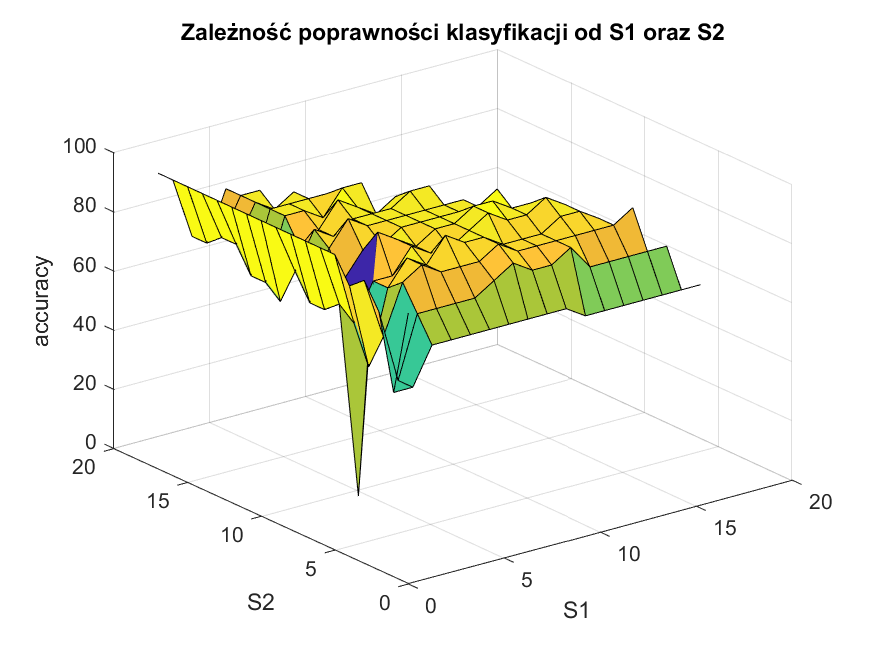
\includegraphics[width=16cm]{figures/S1S2_1.png}
	\caption{Wykres zależności poprawności klasyfikacji od S1 oraz S2 przy lr = 0.2, lr\_inc = 1.05, lr\_dec = 0.9}
	\label{Fig:S1S2_1}
\end{figure}

W przypadku sieci 2-warstwowych, pełną poprawność klasyfikacji zazwyczaj obserwujemy przy mniej niż 1000 epokach, co nie ma miejsca w przypadku sieci 3-warstwowej.
Sieć 3-warstwowa osiągała 100\% poprawność klasyfikacji jedynie w pojedynczych przypadkach.
Może to sugerować że następuje przewymiarowanie sieci i traci ona zdolność uogólniania.
Alternatywnie, możliwym jest także konieczność dłuższego uczenia takiej sieci.
Wizualizację wyników testu widzimy na rysunku \ref{Fig:S1S1_1}.
Podobne wyniki uzyskano dla znacznej większości spośród wszystkich przetestowanych sieci.

Interesujący efekt został natomiast uzyskany dla niskiego wyjścoiwego współczynnika uczenia.
Charakterystyczny dla sieci z niskim współczynnikiem uczenia jest wykres \ref{Fig:S1S2_2}.


\begin{figure}[ht]
	\centering
	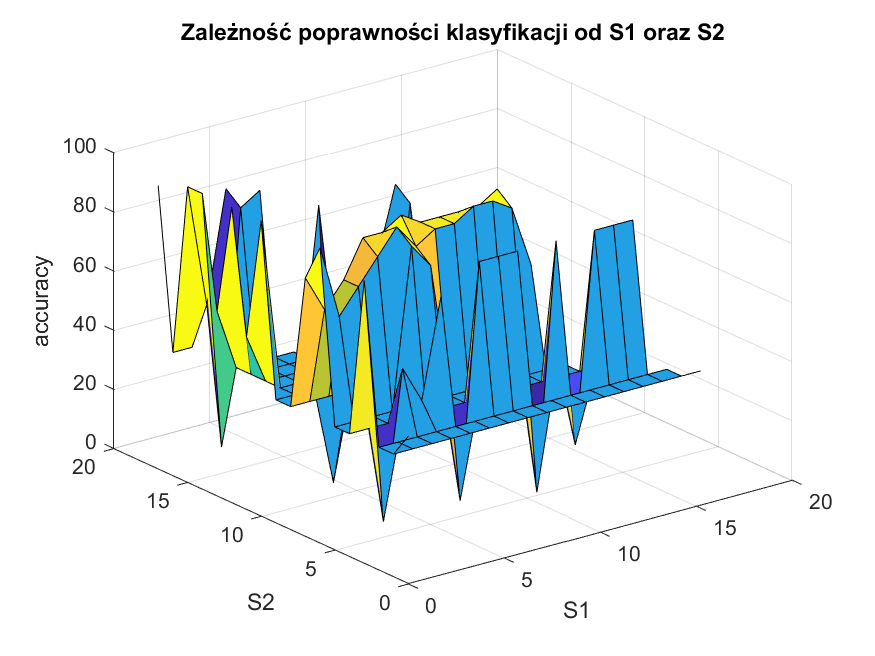
\includegraphics[width=16cm]{figures/S1S2_2.png}
	\caption{Wykres zależności poprawności klasyfikacji od S1 oraz S2 przy lr = 0.0001, lr\_inc = 1.25, lr\_dec = 0.93}
	\label{Fig:S1S2_2}
\end{figure}

W jego przypadku widzimy silną punktowość sieci.
Poprawność klasyfikacji przy niektórych ilościach neuronów w poszczególnych warstwach jest podobna jak w eksperymentach z wyższym współczynnikiem uczenia, zaś w innych spada poniżej 40\%.
Prawdopodobną przyczyną jest duża podatność takiej sieci na parametry początkowe, zwłaszcza dobór wag.
Mimo inicjalizacji generatora pseudolosowego stałym ziarnem, stan wag może być mniej lub bardziej odległy od optymalnego w zależności od liczby neuronów w poszczególnych warstwach.

\clearpage
\subsubsection{Wpływ modyfikatorów współczynnika uczenia na poprawność klasyfikacji}
Poprzez modyfikatory współczynnika uczenia rozumie się parametry lr\_inc oraz lr\_dec, wykorzystywane przy adaptacyjnej aktualizacji współczynnika uczenia.
Powstałe na ich podstawie wykresy pokazują ponadto poziom efektywności sieci o zadanej liczbie neuronów.
Rysunek \ref{Fig:IncDec1} prezentuje rozkład charakterystyczny dla sieci jednowarstwowych

\begin{figure}[ht]
	\centering
	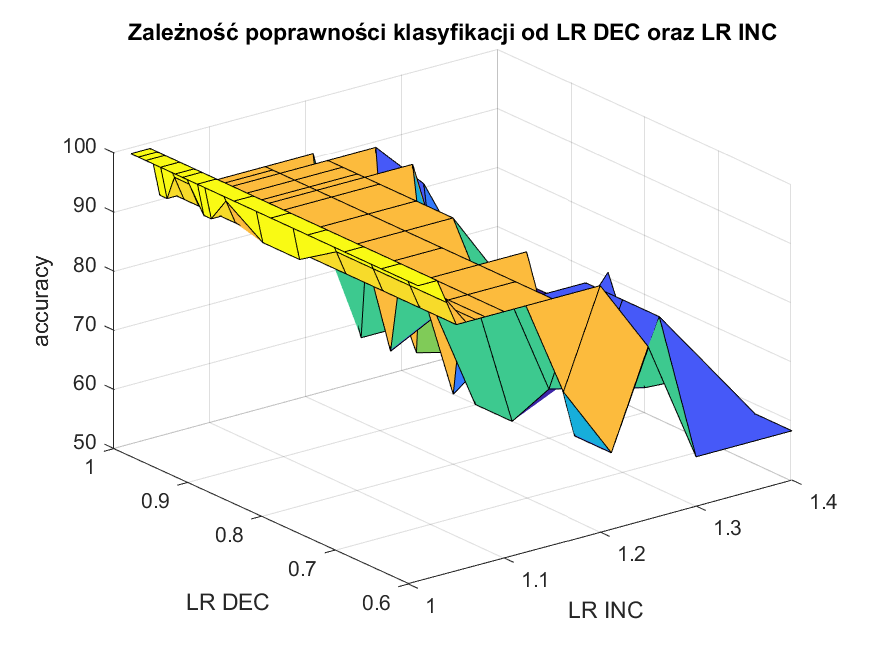
\includegraphics[width=16cm]{figures/IncDec_1.png}
	\caption{Wykres zależności poprawności klasyfikacji od modyfikatorów lr, przy lr~=~0.7 dla sieci jednowarstwowej}
	\label{Fig:IncDec1}
\end{figure}

Widzimy że najlepsza poprawność klasyfikacji wystąpiła dla małych wartości współczynnika lr\_inc.
Współczynnik lr\_dec w tym przypadku nie miał zauważalnego wpływu.
Podobnie w przypadku większości sieci dwuwarstwowych, efekt modyfikatorów był mało zauważalny, co przedstawia rysunek \ref{Fig:IncDec2}.
W tym przypadku jednakże, powodem jest ogólnie duża skuteczność sieci jednowarstwowych.
Większość z nich z łatwością osiąga pełną poprawność klasyfikacji, występują jedynie pojedyncze odchyły bez widocznej zależności.

\begin{figure}[ht]
	\centering
	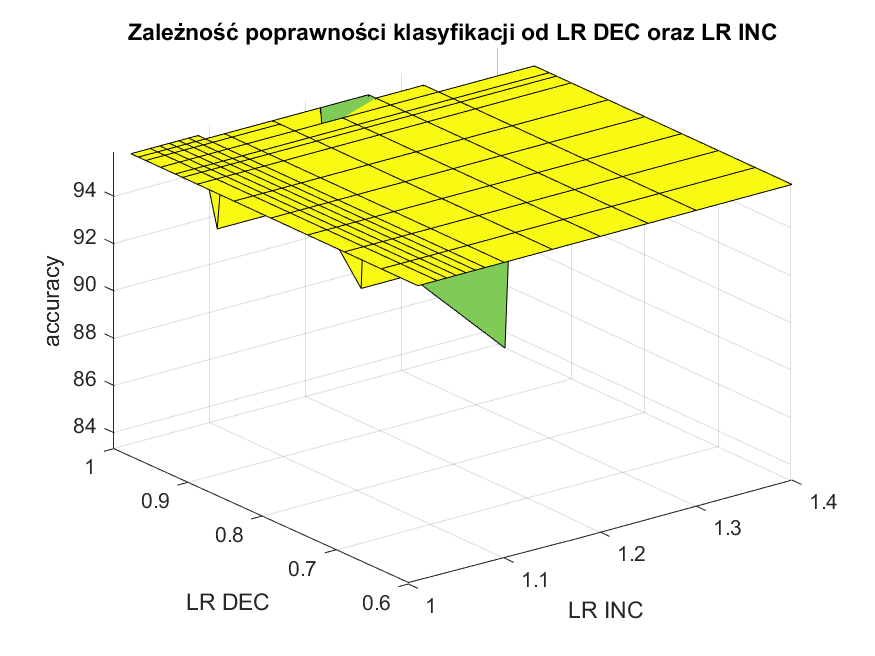
\includegraphics[width=16cm]{figures/IncDec_2.png}
	\caption{Wykres zależności poprawności klasyfikacji od modyfikatorów lr, przy lr~=~0.7 dla sieci dwuwarstwowej przy S1 = 3}
	\label{Fig:IncDec2}
\end{figure}

Interesujące zjawisko możemy jednak zaobserwować przy liczbie neuronów większej od 13, co zaprezentowano na rysunku \ref{Fig:IncDec3}.
W takiej sytuacji, następuje gwałtowny spadek poprawności klasyfikacji przez sieć dwuwarstwową.
Prawdopodobną przyczyną jest przewymiarowanie sieci i jej zbyt duża specjalizacja w klasyfikacji.
W efekcie sieć traci zdolność uogólniającą i nie reaguje poprawnie na dane których nie wykorzystywano podczas uczenia.

\begin{figure}[ht]
	\centering
	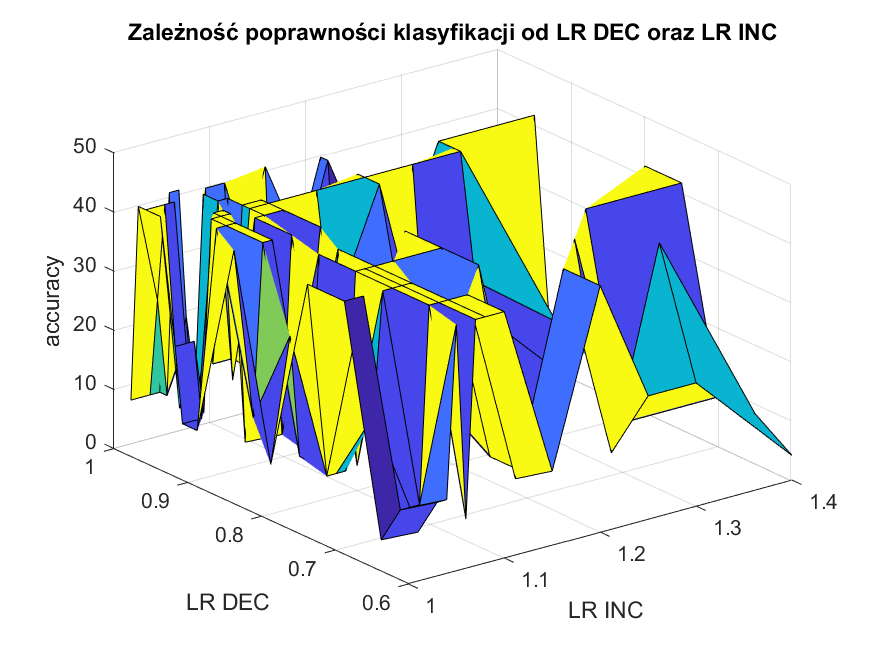
\includegraphics[width=16cm]{figures/IncDec_3.png}
	\caption{Wykres zależności poprawności klasyfikacji od modyfikatorów lr, przy lr~=~0.96 dla sieci dwuwarstwowej przy S1 = 14}
	\label{Fig:IncDec3}
\end{figure}


Również interesujące zjawisko prezentuje rysunek \ref{Fig:IncDec4}.
Widzimy na nim całkowicie stałą poprawność klasyfikacji niezależnie od pozostałych parametrów.
Co więcej, taki wykres występuje wielokrotnie i wyłącznie przy wartościach początkowych współczynnika uczenia mniejszych niż 0,001.
Sugeruje to że wartość taka jest już zbyt mała, i pomimo zastosowania  metody adaptacyjnej sieć nie jest w stanie pokonać minimum lokalnego funkcji błędu, bądź też zadana liczba epok jest zbyt mała aby mogło dojść do efektywnego nauczenia sieci.

\begin{figure}[ht]
	\centering
	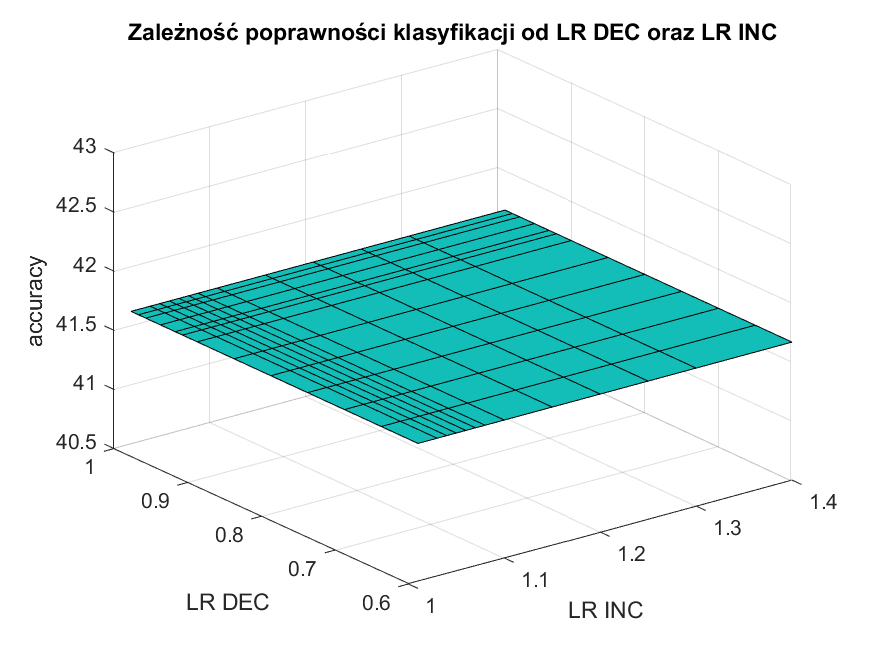
\includegraphics[width=16cm]{figures/IncDec_4.png}
	\caption{Płaski wykres występujący przy niskim początkowym współczynniku uczenia}
	\label{Fig:IncDec4}
\end{figure}

Skuteczność adaptacyjnego współczynnika uczenia objawia się najbardziej w sieciach 3-warstwowych.
Przykładowy wynik uczenia dla takiej sieci obrazuje wykres \ref{Fig:IncDec5}.
W tym przypadku wpływ wartości parametrów adaptacyjnych jest dużo bardziej widoczny niż w poprzednich przykładach.

\begin{figure}[ht]
	\centering
	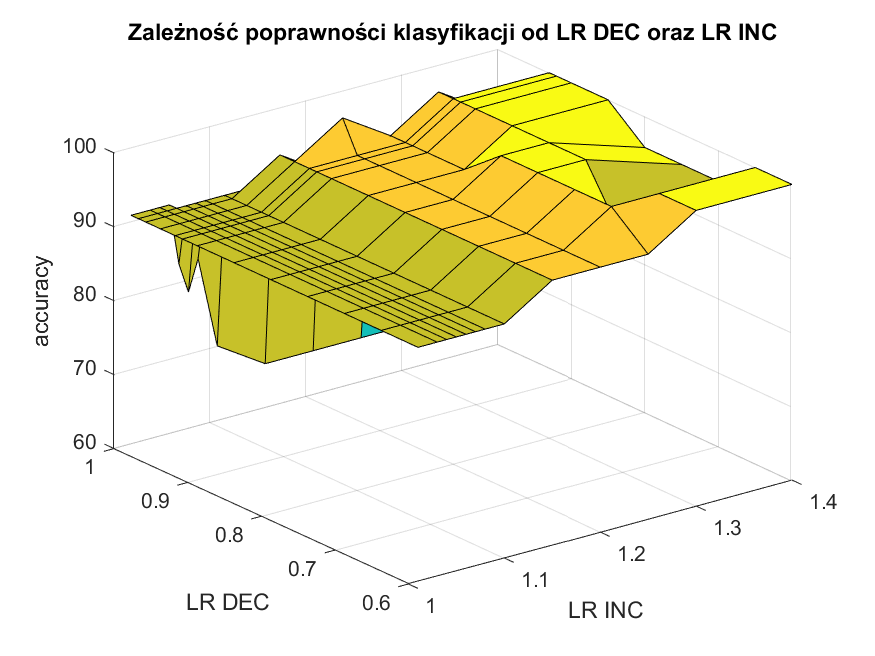
\includegraphics[width=16cm]{figures/IncDec_5.png}
	\caption{Zależność poprawności klasyfikacji od parametrów adaptacyjnych przy lr~=~0.2, S1~=~3 oraz S2~=~10}
	\label{Fig:IncDec5}
\end{figure}

Widzimy że dla osiągnięcia najwyższej skuteczności, istotnym jest ustalenie odpowiedniej wartości obu parametrów.
Jeśli będziemy modyfikować tylko jeden z nich, a drugi pozostawimy bliski jedności, algorytm adaptacyjny wydaje się nie generować zauważalnych zysków.
Warto zauważyć że zwiększenie wartości lr\_inc przy zachowaniu bliskiej jedności wartości lr\_dec przynosi wręcz odwrotny do zamierzonego efekt - poprawność klasyfikacji drastycznie spada.
Zachowanie niskich wartości obydwu współczynników również nie powoduje zauważalnych zmian w procesie uczenia.
Podobne zjawisko widzimy na wykresie \ref{Fig:IncDec6}.
Wprawdzie ze względu na większą liczbę neuronów, sieć osiągnęła pełną poprawność klasyfikacji również dla bliskich jedności wartości współczynników adaptacyjnych, ale zjawisko jej spadku przy złym doborze tych współczynników również jest zauważalne.

\begin{figure}[ht]
	\centering
	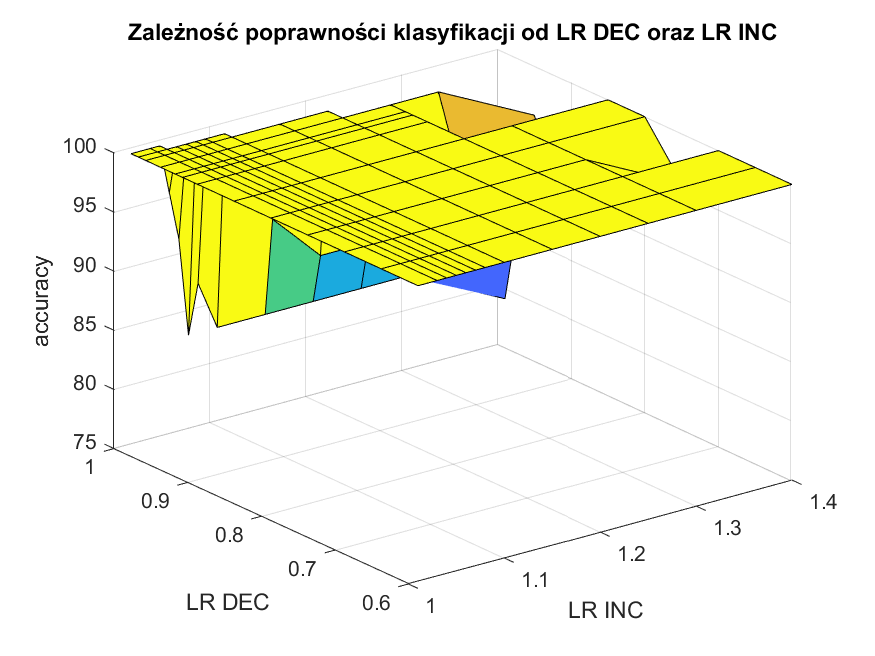
\includegraphics[width=16cm]{figures/IncDec_6.png}
	\caption{Zależność poprawności klasyfikacji od parametrów adaptacyjnych przy lr~=~0.2, S1~=~11 oraz S2~=~5}
	\label{Fig:IncDec6}
\end{figure}

\clearpage
\subsubsection{Wpływ początkowej wartości współczynnika uczenia na proces uczenia}
Badanie to przeprowadzono nadmiarowo, celem określenia najlepszego współczynnika uczenia do przeprowadzenia dalszych testów.
Przykładowy wykres średniej poprawności klasyfikacji dla zadanego współczynnika uczenia w sieci 3-warstwowej prezentują wykresy \ref{Fig:Lr1}

\begin{figure}[ht]
	\centering
	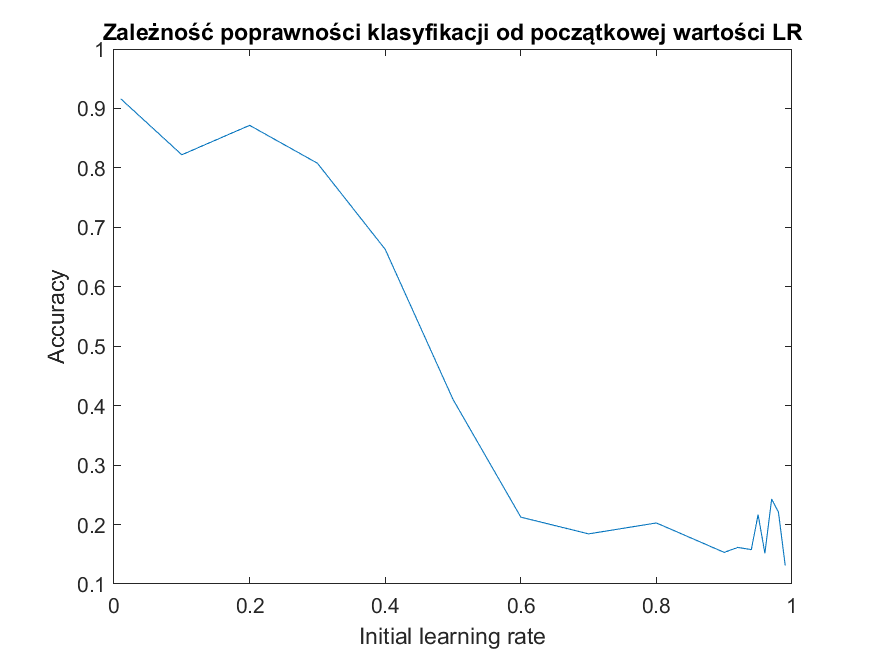
\includegraphics[width=16cm]{figures/Lr1.png}
	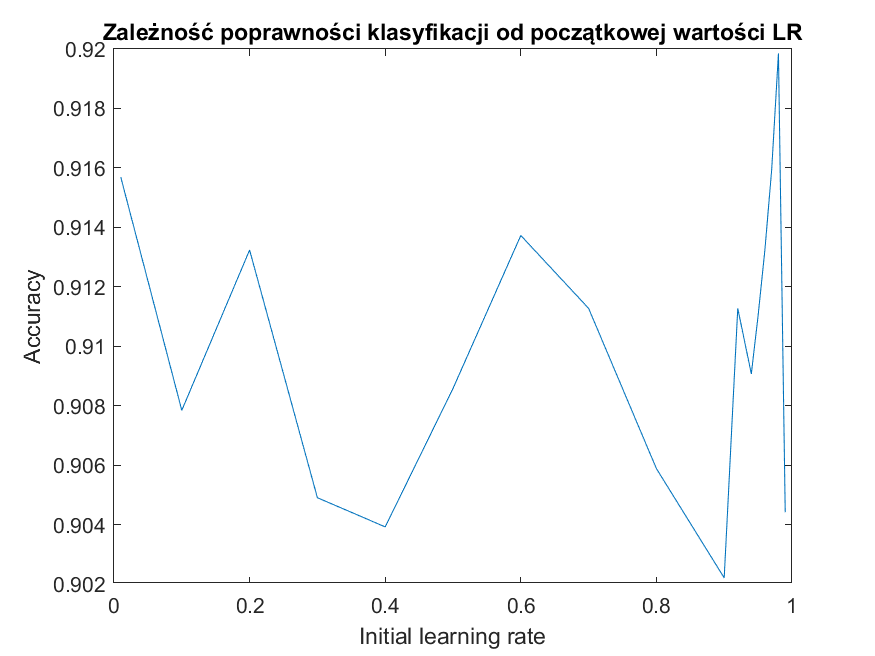
\includegraphics[width=16cm]{figures/Lr2.png}
	\caption{Średnia poprawność klasyfikacji przy S1~=~4, S2~=~7 (wykres górny) oraz S1~=~S2~=~6 (wykres dolny)}
	\label{Fig:Lr1}
\end{figure}
Zauważalna jest zależność, gdzie przy sieci uczącej się ogólnie dobrze, początkowa wartość współczynnika uczenia nie wpływała w znacznym stopniu na poprawność klasyfikacji.
Sieci uczące się gorzej, zwykle najkorzystniej wypadały przy niskim współczynniku uczenia, poniżej wartości 0.4.
Z tego też powodu w kolejnej serii testów przyjęto wartość współczynnika uczenia równą 0.3.

\clearpage
\subsection{Seria 3 - Badanie wpływu parametru błędu granicznego na przebieg oraz wynik procesu uczenia}
W tej serii powtórzono eksperymenty z serii 2, ale przy stałym współczynniku uczenia równym 0.3 i zmiennym współczynnikiem przyrostu błędu adaptacyjnego współczynnika uczenia.
Wykorzystany w tym celu kod prezentuje listing \ref{lst:test2}
W ramach serii wykonano 468 468 testów niezależnych sieci, przy różnych parametrach początkowych.
Podobnie jak w serii drugiej, wagi oraz biasy zainicjowane były stałym ziarnem.

\begin{lstlisting}[language=Rust,caption=Kod wykorzystany do przeprowadzenia 3 serii eksperymentów,label={lst:test2}]
	fn main() {
    //Vector for learning data
    let t_data: Vec<(Array2<f64>, Array2<f64>)>;
    //Vector for validation data
    let v_data: Vec<(Array2<f64>, Array2<f64>)>;

    let data = std::fs::read_to_string("zoo.data");

    let animal_list = data::Animal::new_list(&data.unwrap());
    let animal_list = data::Animal::partitioned_list(animal_list, 0.75);
    t_data = animal_list
        .0
        .iter()
        .map(|a| a.into_training_arr2())
        .collect::<Vec<_>>();

    v_data = animal_list
        .1
        .iter()
        .map(|a| a.into_training_arr2())
        .collect::<Vec<_>>();

    //    dbg!(&t_data);
    let data_len = t_data.len();
    let test_data = v_data
        .iter()
        .map(|(input, output)| {
            (
                input,
                output
                    .iter()
                    .enumerate()
                    .max_by(|(_, a), (_, b)| a.partial_cmp(b).unwrap_or(std::cmp::Ordering::Equal))
                    .unwrap(),
            )
        })
        .map(|(a, s)| (a.clone(), s.0))
        .collect::<Vec<_>>()
        .to_owned();

    println!("Learning record count: {}", t_data.len());
    let lr_step = vec![
        0.0001, 0.001, 0.01, 0.1, 0.2, 0.3, 0.4, 0.5, 0.6, 0.7, 0.8, 0.9, 0.92, 0.94, 0.95, 0.96,
        0.97, 0.98, 0.99, 10.0,
    ];
    let lr_inc_step = vec![
        1.01, 1.03, 1.04, 1.05, 1.06, 1.07, 1.08, 1.1, 1.15, 1.2, 1.25, 1.3, 1.4,
    ];
    let lr_dec_step = vec![
        0.99, 0.98, 0.97, 0.95, 0.93, 0.92, 0.9, 0.85, 0.8, 0.75, 0.7, 0.65, 0.6,
    ];
    let er_step = vec![
        1.0, 1.001, 1.01, 1.02, 1.03, 1.04, 1.05, 1.06, 1.07, 1.08, 1.09, 1.1, 1.15, 1.2, 1.25,
        1.3, 1.4, 1.5,
    ];

    let threads = std::sync::Arc::new(std::sync::Mutex::new(0));
    let (sync_tx, sync_rx) = mpsc::sync_channel(16);
    let (tx, rx) = mpsc::channel();

    let tmp_threads = threads.clone();
    thread::spawn(move || {
        for s1 in 0..t_data.len() / 3 - 7 {
            for s2 in 0..(t_data.len() / 3 - 7 - s1) {
                if s2 == 0 && s1 != 0 {
                    continue;
                }
                let x = Network::new(vec![16, s1, s2, 7]);
                //for lr in &lr_step {
                for er in &er_step {
                    let lr = 0.3;
                    for lr_dec in &lr_dec_step {
                        for lr_inc in &lr_inc_step {
                            let mut net = x.clone();
                            net.name = format!("{},{},{},{},{},{}", s1, s2, lr, lr_dec, lr_inc, er);
                            let mut t_data = t_data.clone();
                            let test_data = test_data.clone();

                            let local_lrs = (lr, *lr_dec, *lr_inc);
                            let local_sync_tx = sync_tx.clone();
                            let local_tx = tx.clone();
                            let local_er = *er;

                            local_sync_tx.send(()).unwrap();
                            let inner_threads = std::sync::Arc::clone(&tmp_threads);

                            *inner_threads.lock().unwrap() += 1;
                            thread::spawn(move || {
                                net.sgd(
                                    &mut t_data,
                                    1000,
                                    data_len,
                                    local_lrs.0,
                                    Some(&test_data),
                                    //None
                                    Some((local_lrs.1, local_lrs.2)),
                                    0.25 / t_data.len() as f64 / 7.0,
                                    1000,
                                    Some(local_er),
                                );
                                local_tx.send(()).unwrap();
                            });
                        }
                    }
                }
            }
        }
    });

    loop {
        let threads = std::sync::Arc::clone(&threads);
        //println!("{}", threads.lock().unwrap());
        rx.recv().unwrap();
        //println!("{}", threads.lock().unwrap());
        sync_rx.recv().unwrap();
        *threads.lock().unwrap() -= 1;
        if *threads.lock().unwrap() <= 0 {
            break;
        }
    }

}
\end{lstlisting}
Jednyną zmianą względem serii pierwszej jest utworzenie nowego wektora przechowującego wartości współczynnika przyrostu błędu granicznego oraz zamiana iteratora lr na er.

\clearpage
\subsubsection{Wpływ zmiennego współczynnika granicznego na poprawność klasyfikacji przy zmiennej liczbie neuronów}
Na bazie uzyskanych w ramach eksperymentów danych, możliwe było ponowne utworzenie wykresów zależności poprawności  klasyfikacji w zależności od liczby neuronów w poszczególnych warstwach sieci.
W przypadku większości wykresów widoczna była wyraźna zależność pomiędzy wartością badanego współczynnika, a ogólną efektywnością sieci.
Dla jego niskich wartości, zbliżonych do jedności, sieć cechowała się silnie niekorzystną charakterystyką, pokazaną na wykresie \ref{Fig:ErS1S21}

\begin{figure}[ht]
	\centering
	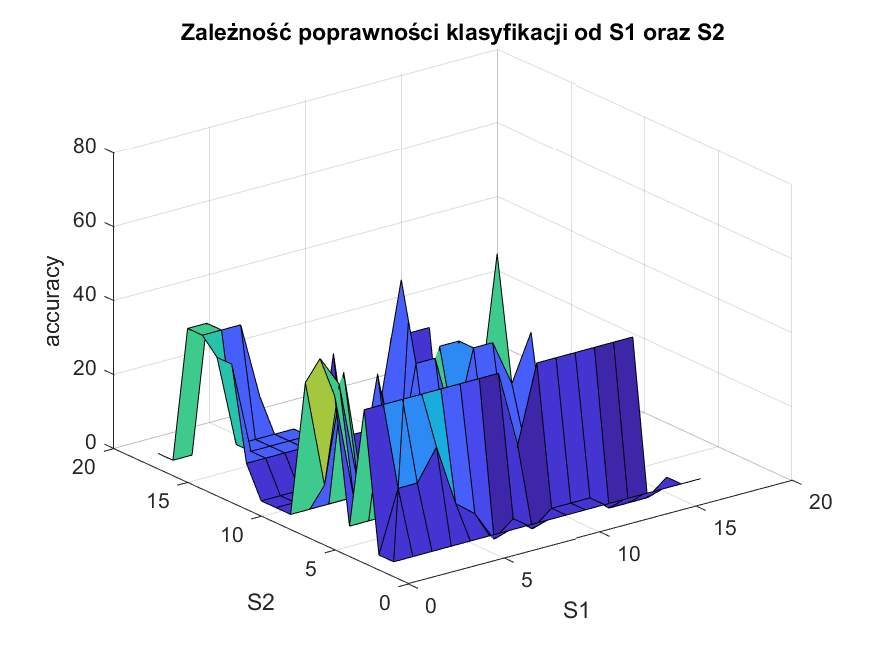
\includegraphics[width=16cm]{figures/ErS1S2_1.png}
	\caption{Poprawność klasyfikacji przy er~=~1, lr\_dec~=~0.8 oraz lr\_inc~=~1.25}
	\label{Fig:ErS1S21}
\end{figure}
Z wykresu wynika, że pomimo teoretycznie bardzo korzystnych wartości współczynników adaptacyjności, niska wartość współczynika błędu granicznego wyraźnie zredukowała zdolność sieci do przeprowadzenia poprawnej klasyfikacji.
Zależność tą dodatkowo popiera kolejny wykres \ref{Fig:ErS1S22} który pokazuje że już niewielkie zwiększenie współczynnika er, znacznie poprawia efektywność uczenia algorytmem adaptacyjnym.
\begin{figure}[ht]
	\centering
	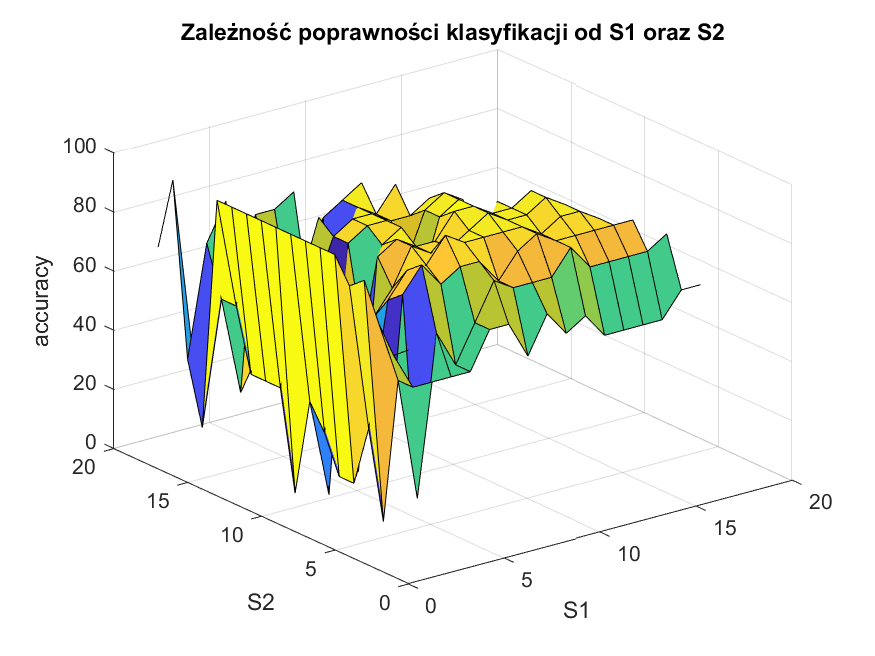
\includegraphics[width=16cm]{figures/ErS1S2_2.png}
	\caption{Poprawność klasyfikacji przy er~=~1.01, lr\_dec~=~0.8 oraz lr\_inc~=~1.25}
	\label{Fig:ErS1S22}
\end{figure}

Istotnym zaznaczenia jest jednakże fakt, że istnieje ryzyko przeszacowania współczynnika er również  w przeciwnym kierunku.
W zależności od pozostałych parametrów adaptacyjnych, jego zwiększanie ponad pewien poziom także spowoduje spadek poprawności klasyfikacji, co prezentuje wykres \ref{Fig:ErS1S23}.
\begin{figure}[ht]
	\centering
	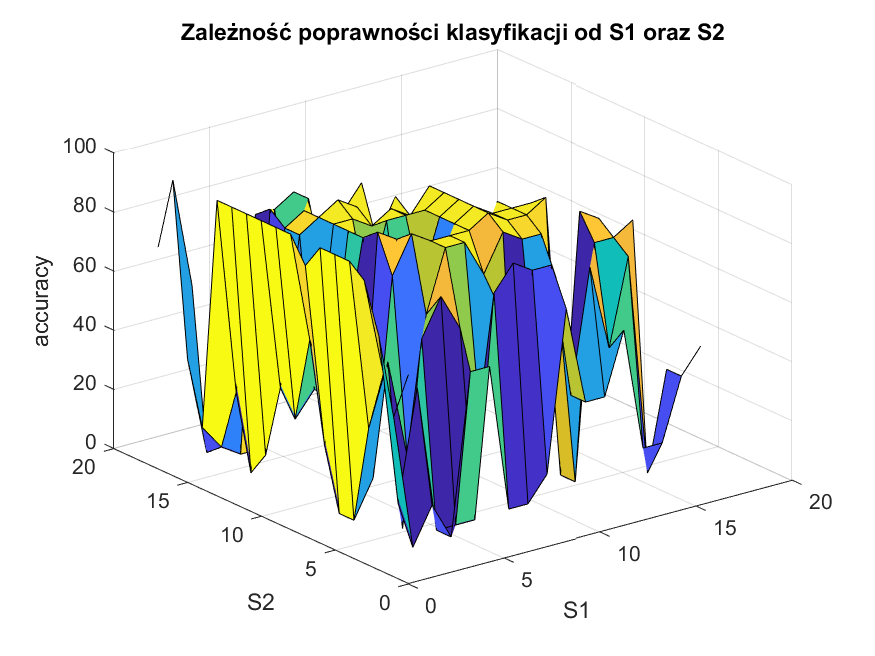
\includegraphics[width=16cm]{figures/ErS1S2_3.png}
	\caption{Poprawność klasyfikacji przy er~=~1.15, lr\_dec~=~0.8 oraz lr\_inc~=~1.25}
	\label{Fig:ErS1S23}
\end{figure}

Trend ten utrzymuje się praktycznie dla wszystkich kombinacji współczynników adaptacyjnych, przy czym zarówno dolna jak i górna granica obszaru efektywnego uczenia nie jest między nimi stała.
Możemy się spodziewać lepszego zobrazowania tego zjawiska w kolejnym zestawieniu.

\clearpage
\subsubsection{Ogólny wpływ parametrów adaptacyjnych na efektywność uczenia sieci}
Poniższe zestawienie pozwala lepiej zaobserwować wpływ parametru er na efektywność uczenia, gdyż przy sieciach o stałej liczbie neuronów, stworzona implementacja gwarantuje w pełni powtarzalne warunki początkowe.
Już wstępna analiza pozyskanych danych pozwala stwierdzić konieczność zastosowania wartości er większej od jedności.
Typowe zachowanie sieci dla przypadku nie spełniającego tego warunku prezentuje wykres \ref{Fig:ErIncDec1}.

\begin{figure}[ht]
	\centering
	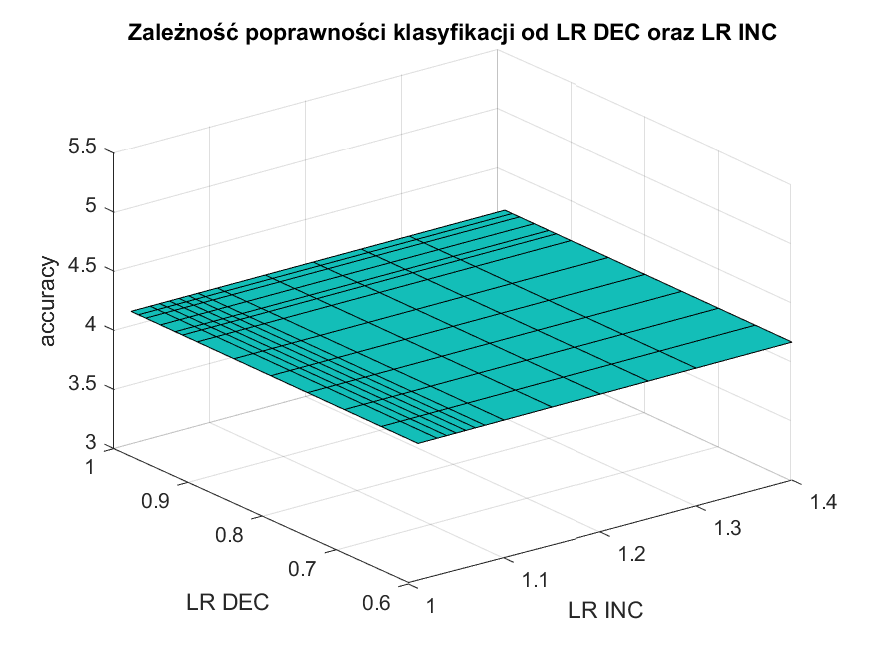
\includegraphics[width=16cm]{figures/ErIncDec_1.png}
	\caption{Poprawność klasyfikacji dla sieci trójwarstwowej przy er~=~1, S1~=~3 oraz S2~=~10}
	\label{Fig:ErIncDec1}
\end{figure}

Co istotne, poprawność klasyfikacji rzędu 4\% jest stanem charakterystycznym dla sieci która nigdy nie podjęła nauki, a jedynie została zainicjalizowana wartościami losowymi.
Może to sugerować błąd warunku brzegowego w wykonanej implementacji algorytmu adaptacyjnego.
Z tej też przyczyny, wyniki dla współczynnika błędu granicznego równego 1 możemy uznać za przypadek odrębny od pozostałych.


Przechodząc do wyników nie należących do przypadku skrajnego, możemy zaobserwować wyraźny wpływ wartości współczynnika błędu granicznego na efektywność uczenia sieci.
Pierwszym przykładem reprezentatywnym jest wykres \ref{Fig:ErIncDec2}.
Pokazuje on przykładową sieć 3-warstwową zdolną do osiągania pełnej poprawności klasyfikacji, ale jednocześnie silnie uzależnioną od doboru metaparametrów.


\begin{figure}[ht]
	\centering
	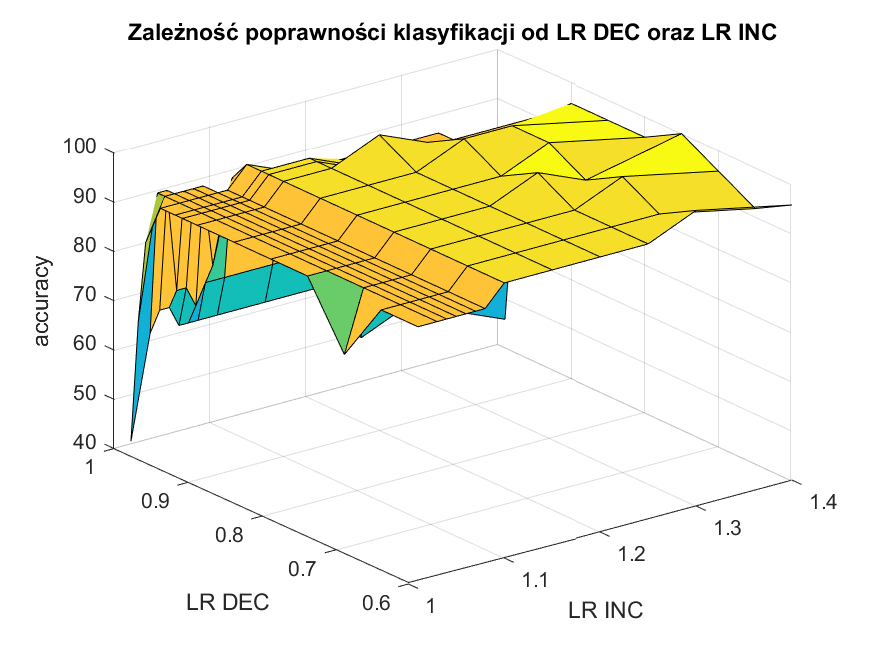
\includegraphics[width=16cm]{figures/ErIncDec_2.png}
	\caption{Poprawność klasyfikacji dla sieci trójwarstwowej przy er~=~1.01, S1~=~3 oraz S2~=~10}
	\label{Fig:ErIncDec2}
\end{figure}

Uwagę warto zwrócić na  występujące również w poprzedniej serii eksperymetnów odchylenia od poziomu średniego dla wartości lr\_dec bliskiej jedności oraz ,,schodkowy'' charakter pozostałej części wykresu.
Wykres \ref{Fig:ErIncDec3} pokazuje wyraźną poprawę zarówno w obszarze dotychczasowo niskiej poprawności, jak i w obszarze najbardziej zbliżonym do pożądanego.
Co więcej, wartości z zakresu 1.04-1.05 wydają się najpotymalniej sprawdzać w większości przypadków sieci, co wyjaśnia zastosowanie ich jako stałych między innymi w środowisku MATLAB.

\begin{figure}[ht]
	\centering
	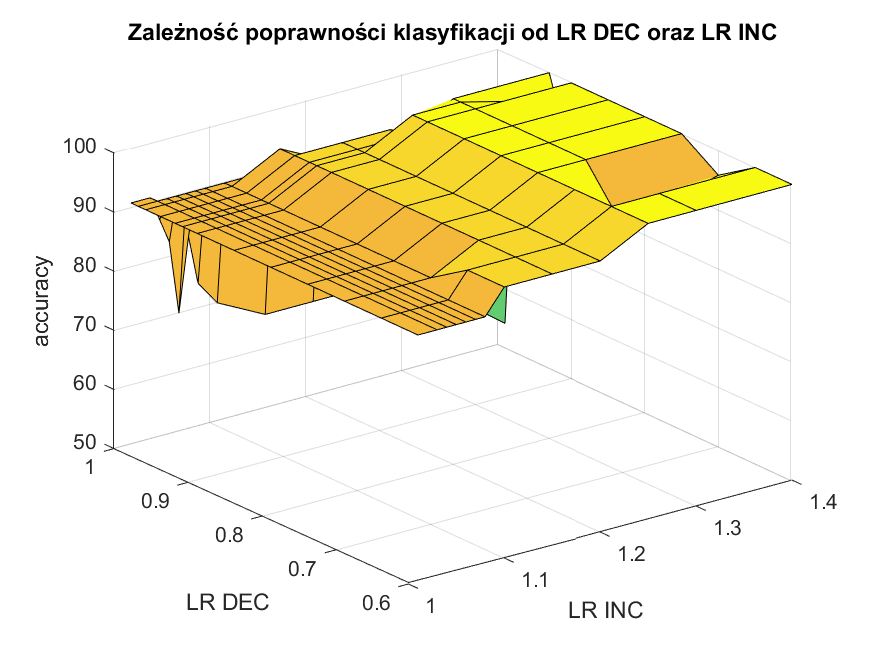
\includegraphics[width=16cm]{figures/ErIncDec_3.png}
	\caption{Poprawność klasyfikacji dla sieci trójwarstwowej przy er~=~1.04, S1~=~3 oraz S2~=~10}
	\label{Fig:ErIncDec3}
\end{figure}

W przypadku tej konfiguracji sieci dalsze zwiększanie wartości er nie powoduje silnego spadku poprawności klasyfikacji.
Co więcej, dla jego wysokich wartości dochodzi do zaniku ,,schodkowego'' charakteru rozkładu poprawności klasyfikacji, co prezentuje wykres \ref{Fig:ErIncDec4}.
Należy jednak zwrócić uwagę, że pomimo ogólnej poprawy działania sieci o zadanej liczbie neuronów, zanika jej zdolność do osiągania pełnej poprawności.
Widoczne są jednak pojedyncze sukcesy w jej osiągnięciu, a sama sieć wydaje się posiadać względnie dobrą zdolność uogólniającą.
Możliwe że zwiększenie liczby epok, wpłynęłoby pozytywnie na wyniki procesu uczenia.

\begin{figure}[ht]
	\centering
	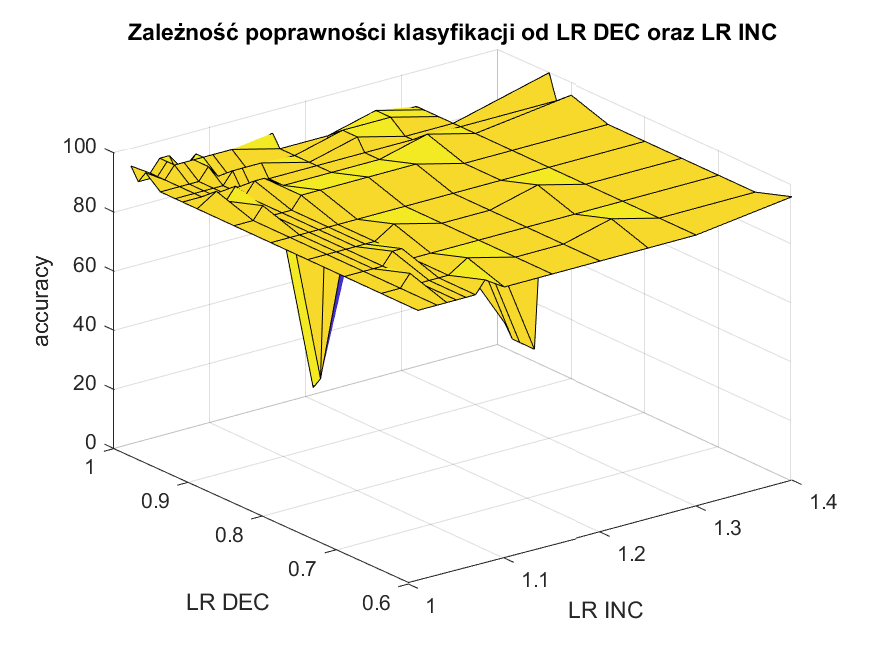
\includegraphics[width=16cm]{figures/ErIncDec_4.png}
	\caption{Poprawność klasyfikacji dla sieci trójwarstwowej przy er~=~1.5, S1~=~3 oraz S2~=~10}
	\label{Fig:ErIncDec4}
\end{figure}


\clearpage
\subsubsection{Uogólniony wpływ współczynnika błędu granicznego na poprawność klasyfikacji}
Na podstawie przeprowadzonych eksperymentów, podobnie jak w serii drugiej, możliwa była również obserwacja wpływu parametru er na średnią efektywność uczenia każdej z testowanych sieci.
W przypadku sieci 2 warstwowej zauważalny był ogólny stały trend zaprezentowany na wykresie \ref{Fig:Er1}.

\begin{figure}[ht]
	\centering
	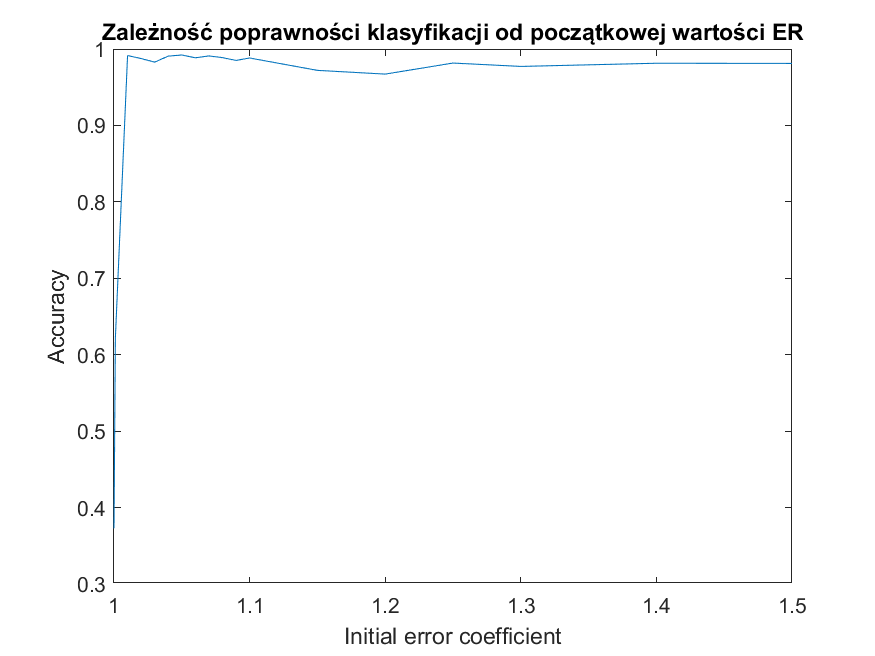
\includegraphics[width=16cm]{figures/Er_1.png}
	\caption{Średnia poprawność klasyfikacji sieci 2-warstwowej przy 13 neuronach w warstwie pierwszej}
	\label{Fig:Er1}
\end{figure}

Sieci 2-warstwowe utrzymywały ogólnie dobrą poprawność klasyfikacji niezależnie od wartości współczynnika er.
Co więcej, również przy obecnie przyjętej reprezentacji wyników widoczny jest drastyczny spadek poprawności klasyfikacji dla współczynnika równego jedności.
Jest to kolejna przesłanka świadcząca o możliwym błędzie implementacji dla tego warunku brzegowego.

W przypadku sieci 3-warstwowych występują 2 ogólne trendy.
Pierwszy podobny do trendu dla sieci 2-warstwowych prezentuje wykres \ref{Fig:Er2}.

\begin{figure}[ht]
	\centering
	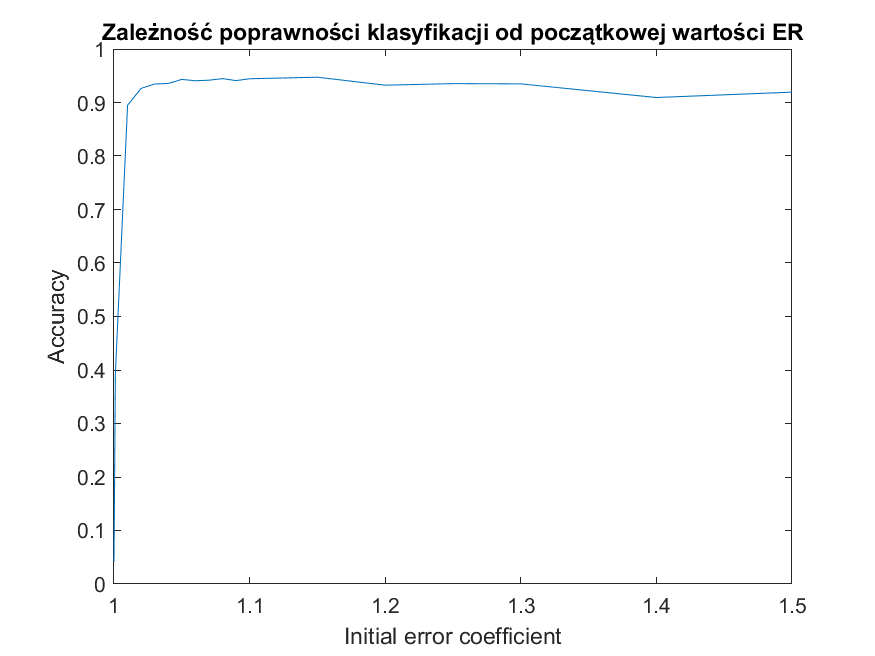
\includegraphics[width=16cm]{figures/Er_2.png}
	\caption{Średnia poprawność klasyfikacji sieci 3-warstwowej przy S1~=~5 oraz S2~=~10}
	\label{Fig:Er2}
\end{figure}

Jest to zachowanie typowe dla sieci o względnie dużej liczbie neuronów w dwóch pierwszych warstwach.
Wskazuje to na ogólnie dobrą efektywność takich sieci, i idący za tym szeroki zakres korzystnych wartości współczynnika er.
Reguła ta nie jest jednak stała, i objawia się przede wszystkim w sieciach o mniejszej liczbie neuronów a także w sieciach w których występuje wysoka dysproporcja liczby neuronów między wartstwą pierwszą oraz drugą.
Przykład alternatywnego trendu widzimy na wykresie \ref{Fig:Er3}.

\begin{figure}[ht]
	\centering
	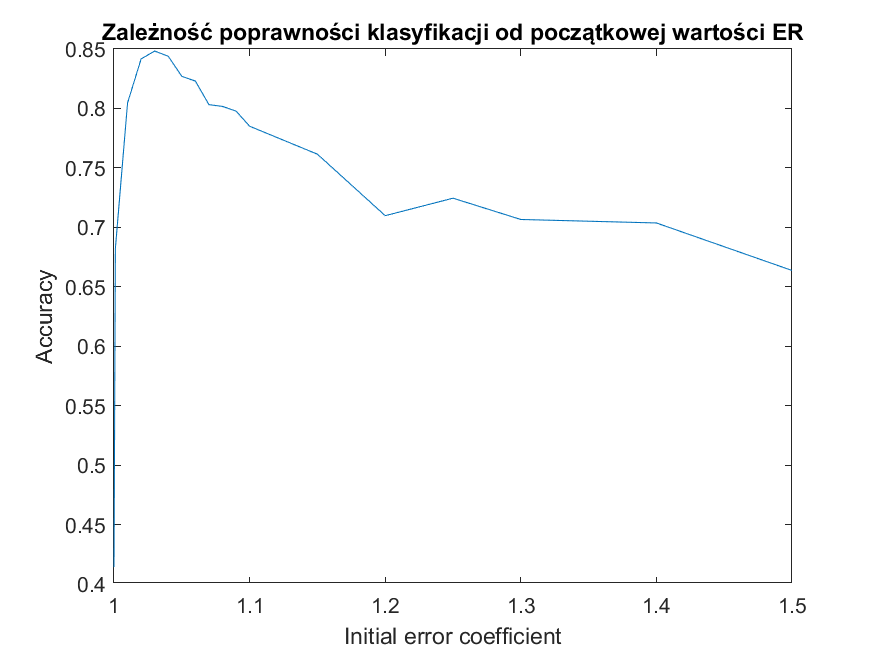
\includegraphics[width=16cm]{figures/Er_3.png}
	\caption{Średnia poprawność klasyfikacji sieci 3-warstwowej przy S1~=~11 oraz S2~=~3}
	\label{Fig:Er3}
\end{figure}

Sieci takie cechowały się przede wszystkim ogólnie gorszą średnią poprawnością klasyfikacji, rzadko osiągającą ponad 85\%.
W ich przypadku, najlepszą efektywność uzyskiwano przy niskich wartościach współczynnika błędu granicznego.
Podobnie jak wnioskowano na podstawie wykresów zależności poprawności klasyfikacji od współczynników adaptacyjnych,
również w tym przypadku widzimy że najlepszą efektywność w przypadku takich sieci uzyskuje się dla wartości er bliskich 1.05.

\clearpage

\subsubsection{Seria 4 oraz seria 5 - Testy metody stochastycznej}
Celem tej serii eksperymentów była weryfikacja korzyści płynących z zastosowania metody stochastycznej.
W celu zapewnienia lepszych możliwości porównawczych wykonano pewne modyfikacje względem eksperymentów z poprzednich serii, co wymusiło również wykonanie niestochastycznej próby kontrolnej.
Wprowadzone zmiany to:
\begin{itemize}
	\item Zmniejszenie liczby testowanych sieci do 75 460.
	\item Zwiększenie wartości błędu docelowego do teoretycznie wystarczającego, lecz mniej efektywnego poziomu.
	\item Zwiększenie limitu epok do 10 000.
	\item Przyjęcie wartości współczynników z nisko efektywnych zakresów
\end{itemize}

Do przeprowadzenia eksperymentów wkorzystano kod przedstawiony na listingu \ref{lst:test3}
\begin{lstlisting}[language=Rust,caption=Kod wykorzystany do przeprowadzenia 3 serii eksperymentów,label={lst:test3}]
	fn main() {
    //Vector for learning data
    let t_data: Vec<(Array2<f64>, Array2<f64>)>;
    //Vector for validation data
    let v_data: Vec<(Array2<f64>, Array2<f64>)>;

    let data = std::fs::read_to_string("zoo.data");

    let animal_list = data::Animal::new_list(&data.unwrap());
    let animal_list = data::Animal::partitioned_list(animal_list, 0.75);
    t_data = animal_list
        .0
        .iter()
        .map(|a| a.into_training_arr2())
        .collect::<Vec<_>>();

    v_data = animal_list
        .1
        .iter()
        .map(|a| a.into_training_arr2())
        .collect::<Vec<_>>();

    //    dbg!(&t_data);
    let data_len = t_data.len();
    let test_data = v_data
        .iter()
        .map(|(input, output)| {
            (
                input,
                output
                    .iter()
                    .enumerate()
                    .max_by(|(_, a), (_, b)| a.partial_cmp(b).unwrap_or(std::cmp::Ordering::Equal))
                    .unwrap(),
            )
        })
        .map(|(a, s)| (a.clone(), s.0))
        .collect::<Vec<_>>()
        .to_owned();

    println!("Learning record count: {}", t_data.len());
    let lr_step = vec![
        0.0001, 0.001, 0.01, 0.1, 0.2, 0.3, 0.4, 0.5, 0.6, 0.7, 0.8, 0.9, 0.92, 0.94, 0.95,
    ];
    let lr_inc_step = vec![
        1.05, 1.06, 1.07, 1.08, 1.1, 1.15, 1.2, 1.25,
    ];
    let lr_dec_step = vec![
        0.95, 0.93, 0.92, 0.9, 0.85, 0.8, 0.75, 0.7
    ];
    let er_step = vec![
        1.0, 1.001, 1.01, 1.02, 1.03, 1.04, 1.05, 1.06, 1.07, 1.08
    ];

    let threads = std::sync::Arc::new(std::sync::Mutex::new(0));
    let (sync_tx, sync_rx) = mpsc::sync_channel(16);
    let (tx, rx) = mpsc::channel();

    let tmp_threads = threads.clone();
    thread::spawn(move || {
        for s1 in 0..t_data.len() / 3 - 7 {
            for s2 in 0..(t_data.len() / 3 - 7 - s1) {
                if s2 == 0 && s1 != 0 {
                    continue;
                }
                let x = Network::new(vec![16, s1, s2, 7]);
                //for lr in &lr_step {
                for er in &er_step {
                    let lr = 0.3;
                    for lr_dec in &lr_dec_step {
                        for lr_inc in &lr_inc_step {
                            let mut net = x.clone();
                            net.name = format!("{},{},{},{},{},{}", s1, s2, lr, lr_dec, lr_inc, er);
                            let mut t_data = t_data.clone();
                            let test_data = test_data.clone();

                            let local_lrs = (lr, *lr_dec, *lr_inc);
                            let local_sync_tx = sync_tx.clone();
                            let local_tx = tx.clone();
                            let local_er = *er;

                            local_sync_tx.send(()).unwrap();
                            let inner_threads = std::sync::Arc::clone(&tmp_threads);

                            *inner_threads.lock().unwrap() += 1;
                            thread::spawn(move || {
                                net.sgd(
                                    &mut t_data,
                                    10000,
                                    //data_len, //Próba kontrolna
                                    data_len / 2, //Rozmiar próbek równy połowie długości całego zbioru uczącego
                                    local_lrs.0,
                                    Some(&test_data),
                                    //None
                                    Some((local_lrs.1, local_lrs.2)),
                                    0.25 / data_len as f64,
                                    10000,
                                    Some(local_er),
                                );
                                local_tx.send(()).unwrap();
                            });
                        }
                    }
                }
            }
        }
    });

    loop {
        let threads = std::sync::Arc::clone(&threads);
        //println!("{}", threads.lock().unwrap());
        rx.recv().unwrap();
        //println!("{}", threads.lock().unwrap());
        sync_rx.recv().unwrap();
        *threads.lock().unwrap() -= 1;
        if *threads.lock().unwrap() <= 0 {
            break;
        }
    }

}
\end{lstlisting}

Zgodnie z oczekiwaniami sieć wzorcowa osiągnęła względnie niską efektywność uczenia, co widać na wykresie \ref{Fig:Stoch1}.

\begin{figure}[ht]
	\centering
	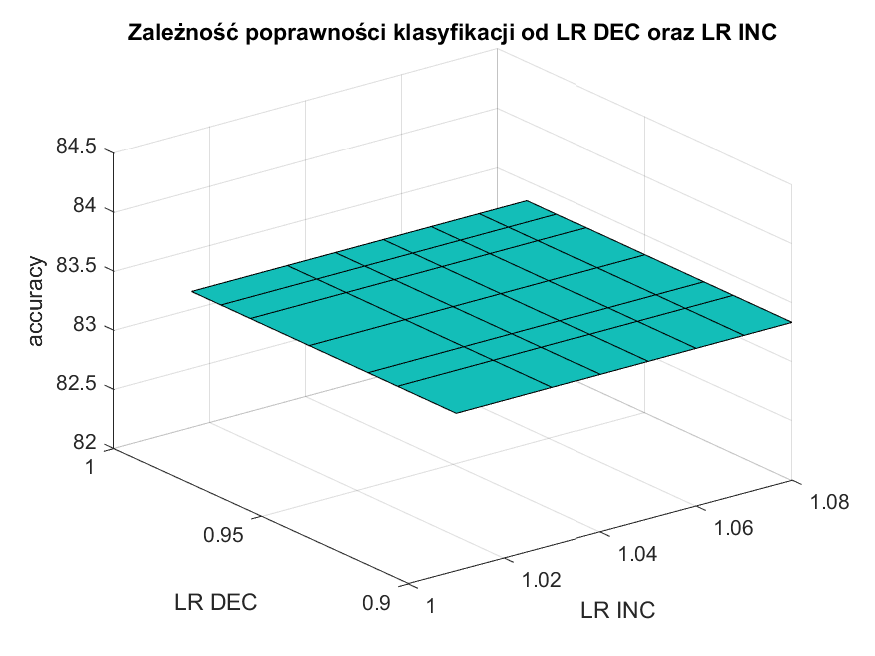
\includegraphics[width=16cm]{figures/Stoch_1.png}
	\caption{Poprawność klasyfikacji sieci 3-warstwowej przy er~=~1.07 S1~=~4 oraz S2~=~10}
	\label{Fig:Stoch1}
\end{figure}
Taki stan jest korzystny dla eksperymentu, gdyż pozwoli na zaobserwowanie zarówno ewentualnej poprawy jak i pogorszenia poprawności klasyfikacji.


Na przestrzeni eksperymentu odnotowano jedynie pojedyncze różnice pomiędzy siecią uczoną metodą stochastyczną a podstawowym algorytmem.
W trakcie procesu uczenia zaobserwowano jednak dużo krótszy czas zakończenia serii, co sugeruje szybsze osiąganie przez taką sieć docelowego błędu.
Niestety, w raporcie testowym nie zapisywano liczby epok wykonanych w procesie uczenia sieci, co uniemożliwia wykonanie porównania bez
Porównanie takie byłoby dobrym sposobem porównania metody stochastycznej z domyślnym algorytmem, gdyż pod względem poprawności klasyfikacji różnice między nimi są pomijalne, co w przypadku sieci z wykresu \ref{Fig:Stoch1} prezentuje wykres \ref{Fig:Stoch2}.

\begin{figure}[ht]
	\centering
	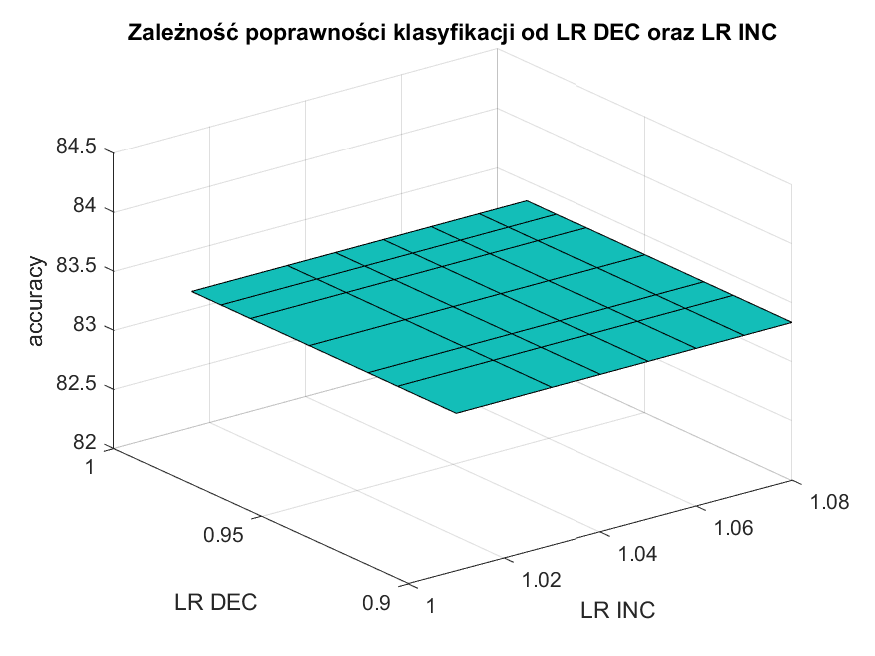
\includegraphics[width=16cm]{figures/Stoch_2.png}
	\caption{Poprawność klasyfikacji sieci 3-warstwowej uczonej metodą stochastyczną przy er~=~1.07 S1~=~4 oraz S2~=~10}
	\label{Fig:Stoch2}
\end{figure}


\clearpage
\subsection{Seria 6 - testy osłabionego algorytmu adaptacyjnego}
Poprzez osłabienie algorytmu adaptacyjnego rozumie się pozbawienie go zdolności do przywrócenia korzystniejszych wartości wag oraz biasów po przekroczeniu granicznego przyrostu błędu.
Zmianę w kodzie wymaganą do wykonania tego testu prezentuje listing \ref{lst:Retarded0}
\begin{lstlisting}[language=Rust,caption=Fragment funkcji sgd\(...\) - zakomentowanie linii przywracających zachowane wagi oraz biasy,label={lst:Retarded0}]
	Some((dec, inc)) => {
		// Saving state of network before readjustment of weights and biases
		let saved_weights = self.weights.clone();
		let saved_biases = self.biases.clone();
		let previous_error = self.mse(training_data);

		//Sub-loob performing learning step for each of the mini-batch
		for mini_batch in &mut mini_batches {
			//dbg!(&mini_batch);
			self.update_mini_batch(mini_batch, eta, batch_count)
		}

		// Verification of newly achieved Mean Square Error
		let new_error = self.mse(training_data);
		if new_error < target_cost {
			if let Some(data) = &test_data {
				let output = self.evaluate(data);
				println!("{},{}", self.name, output.1 as f64 / output.0 as f64);
			}
			break;
		}
		if new_error
			> previous_error
				* if let Some(perf_inc) = er {
					perf_inc
				} else {
					MAX_PERF_INC
				}
		{
			// Restoring backup

			//Linie zakomentowane na potrzeby eksperymentu
			//self.weights = saved_weights;
			//self.biases = saved_biases;

			// Adaptation - learning rate decreases
			eta *= dec;
		} else if new_error < previous_error {
			// Adaptation - learning rate increases
			eta *= inc;
		}
		// else statement does nothing - ommited
	}
\end{lstlisting}
Przywrócenie to powoduje inwalidację obliczonych w poprzedniej iteracji algorytmu parametrów, co może być uznane za niepotrzebne poświęcanie czasu na dodatkowe obliczenia.
Wrażenie to jest jednak mylne, co widzimy na wykresie \ref{Fig:Retarded1}.

\begin{figure}[ht]
	\centering
	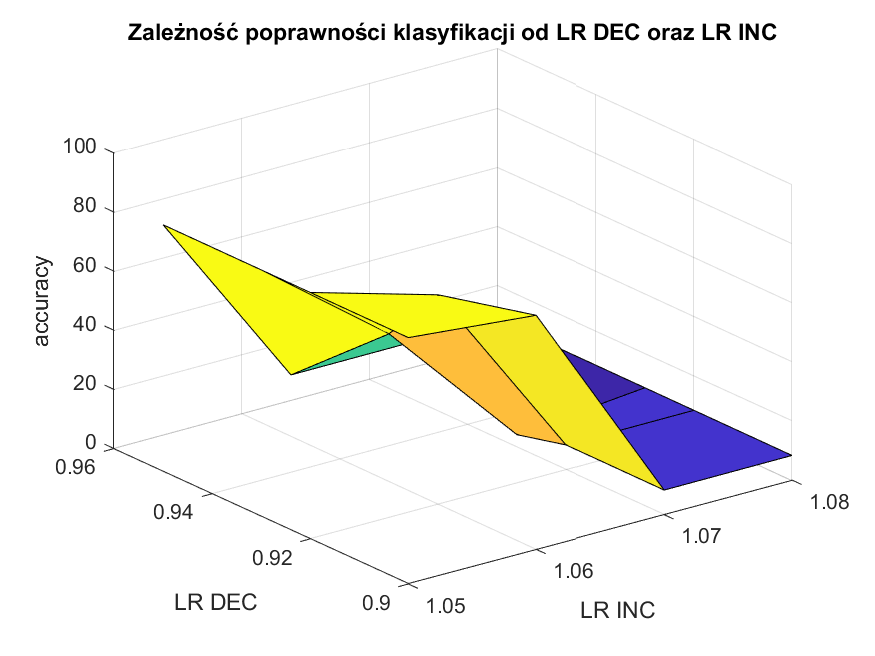
\includegraphics[width=16cm]{figures/Retarded_1.png}
	\caption{Poprawność klasyfikacji sieci 3-warstwowej uczonej przy  przy er~=~1.07 S1~=~4 oraz S2~=~10}
	\label{Fig:Retarded1}
\end{figure}
Co istotne, widzimy dużo mniejszą rozdzielczość wartości metaparametrów dla których testowano sieć.
Jest to spowodowane drastycznym spadkiem wydajności procesu uczenia takiej sieci.
Spadek ten jest na tyle drastyczny że pomimo redukcji liczby testów do zaledwie kilkunastu tysięcy, podobniej jak w seriach 4 oraz 5, proces uczenia przy maksymalnej liczbie epok równej 10000 i względnie wysokim błędzie docelowym równym $0.25/\text{len}(\text{dataset})$ trwał około 30 godzin.
W przypadku eksperymentów serii 4 oraz 5, w których badano większą liczbę sieci lecz przy tych samych parametrach startowych wynosił on nie więcej niż 5 godzin, zaś w seriach 2 oraz 3 w których badano znacznie więcej sieci, lecz przy niższym limicie epok, wynosił około 8 godzin.

Dysproporcje czasowe występukjące w przypadku tej serii eksperymentów były na tyle znaczące że zdecydowano się na wykonanie pojedynczych eksperymentów z bardziej szczegółowym raportem, pozwalających na bardziej dokładne zbadanie zachowania sieci.
W celu przeprowadzenia dodatkowego eksperymentu przyjęto parametry przedstawione na listingu \ref{lst:Retarded1}.

\begin{lstlisting}[language=Rust,caption=Kod wykorzystany do przeprowadzenia dodatkowego eksperymentu w serii 6,label={lst:Retarded1}]
	fn main() {
    println!("Hello, world!");
    //let x = Network::new(vec![16, 8, 7]);

    //dbg!(&x);
    //dbg!(x.backprop(&Array2::<f64>::zeros((2, 1)), &Array2::<f64>::zeros((4, 1))));

    //Vector for learning data
    let t_data: Vec<(Array2<f64>, Array2<f64>)>;
    //Vector for validation data
    let v_data: Vec<(Array2<f64>, Array2<f64>)>;

    let data = std::fs::read_to_string("zoo.data");

    let animal_list = data::Animal::new_list(&data.unwrap());
    let animal_list = data::Animal::partitioned_list(animal_list, 0.75);
    t_data = animal_list
        .0
        .iter()
        .map(|a| a.into_training_arr2())
        .collect::<Vec<_>>();

    v_data = animal_list
        .1
        .iter()
        .map(|a| a.into_training_arr2())
        .collect::<Vec<_>>();

    //    dbg!(&t_data);
    let data_len = t_data.len();
    let test_data = v_data
        .iter()
        .map(|(input, output)| {
            (
                input,
                output
                    .iter()
                    .enumerate()
                    .max_by(|(_, a), (_, b)| a.partial_cmp(b).unwrap_or(std::cmp::Ordering::Equal))
                    .unwrap(),
            )
        })
        .map(|(a, s)| (a.clone(), s.0))
        .collect::<Vec<_>>()
        .to_owned();

    println!("Learning record count: {}", t_data.len());
//    let lr_step = vec![
//        0.0001, 0.001, 0.01, 0.1, 0.2, 0.3, 0.4, 0.5, 0.6, 0.7, 0.8, 0.9, 0.92, 0.94, 0.95,
//    ];
    let lr_inc_step = vec![
        1.01, 1.03, 1.04, 1.05, 1.06, 1.07, 1.08, 1.1, 1.15, 1.2, 1.25, 1.3, 1.4
    ];
    let lr_dec_step = vec![
        0.99, 0.98, 0.97, 0.95, 0.93, 0.92, 0.9, 0.85, 0.8, 0.75, 0.7, 0.65, 0.6
    ];

//    let er_step = vec![
//        1.0, 1.001, 1.01, 1.02, 1.03, 1.04, 1.05, 1.06, 1.07, 1.08
//    ];

    let threads = std::sync::Arc::new(std::sync::Mutex::new(0));
    let (sync_tx, sync_rx) = mpsc::sync_channel(16);
    let (tx, rx) = mpsc::channel();

    let tmp_threads = threads.clone();
    thread::spawn(move || {
        //for s1 in 0..t_data.len() / 3 - 7 {
            //for s2 in 0..(t_data.len() / 3 - 7 - s1) {
                //if s2 == 0 && s1 != 0 {
                //    continue;
                //}
        let (s1, s2) = (4,10);
        let x = Network::new(vec![16, s1, s2, 7]);
        //for lr in &lr_step {
        //for er in &er_step {
            let er = 1.07;
            let lr = 0.3;
            for lr_dec in &lr_dec_step {
                for lr_inc in &lr_inc_step {
                    let mut net = x.clone();
                    net.name = format!("{},{},{},{},{},{}", s1, s2, lr, lr_dec, lr_inc, er);
                    let mut t_data = t_data.clone();
                    let test_data = test_data.clone();

                    let local_lrs = (lr, *lr_dec, *lr_inc);
                    let local_sync_tx = sync_tx.clone();
                    let local_tx = tx.clone();
                    let local_er = er;

                    local_sync_tx.send(()).unwrap();
                    let inner_threads = std::sync::Arc::clone(&tmp_threads);

                    *inner_threads.lock().unwrap() += 1;
                    thread::spawn(move || {
                        net.sgd(
                            &mut t_data,
                            10000,
                            data_len ,
                            local_lrs.0,
                            Some(&test_data),
                            //None
                            Some((local_lrs.1, local_lrs.2)),
                            0.25 / data_len as f64 / 7.0,
                            10000,
                            Some(local_er),
                        );
                        local_tx.send(()).unwrap();
                    });
                }
    //}
    //}
    //}
        }
    });

    loop {
        let threads = std::sync::Arc::clone(&threads);
        //println!("{}", threads.lock().unwrap());
        rx.recv().unwrap();
        //println!("{}", threads.lock().unwrap());
        sync_rx.recv().unwrap();
        *threads.lock().unwrap() -= 1;
        if *threads.lock().unwrap() <= 0 {
            break;
        }
    }

}
\end{lstlisting}

Przeprowadzony test pozwolił na porównanie zachowania pierwotnej i osłabionej wersji algorytmu.
Ze względu na przeprowadzoną przed serią 4 modyfikację sposobu uziarniania generatora pseudolosowego, wyniki uczenia  są różne od tych otrzymanych w seriach 2 oraz 3, lecz nadal zachowują ogólny obserwowany w nich trend.
Próbę kontrolną, dla dotychczasowego algorytmu prezentuje wykres \ref{Fig:Retarded2}.

\begin{figure}[ht]
	\centering
	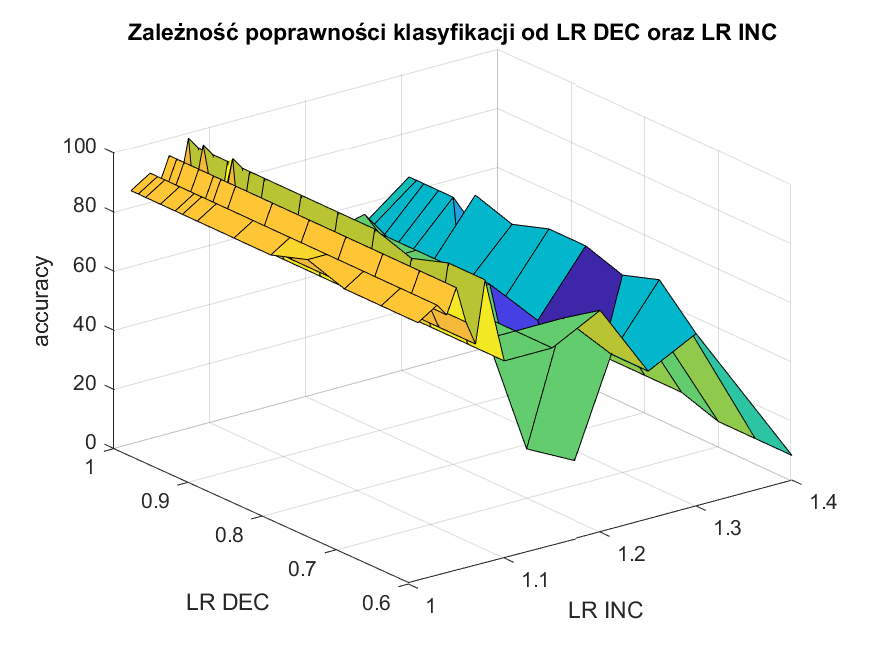
\includegraphics[width=16cm]{figures/Retarded_2.png}
	\caption{Poprawność klasyfikacji sieci uczonej standardowym algorytmem przy er~=~1.07 S1~=~4 oraz S2~=~10}
	\label{Fig:Retarded2}
\end{figure}
Na wykresie widzimy podatność poprawności klasyfikacji głównie na zmiany współczynnika lr\_inc.
Trend ten jest zachowany również w przypadku osłabionego algorytmu.
Jednakże jak zaprezentowano na wykresie \ref{Fig:Retarded3} spadki poprawności klasyfikacji dla niekorzystnych parametrów są znacznie większe.

\begin{figure}[ht]
	\centering
	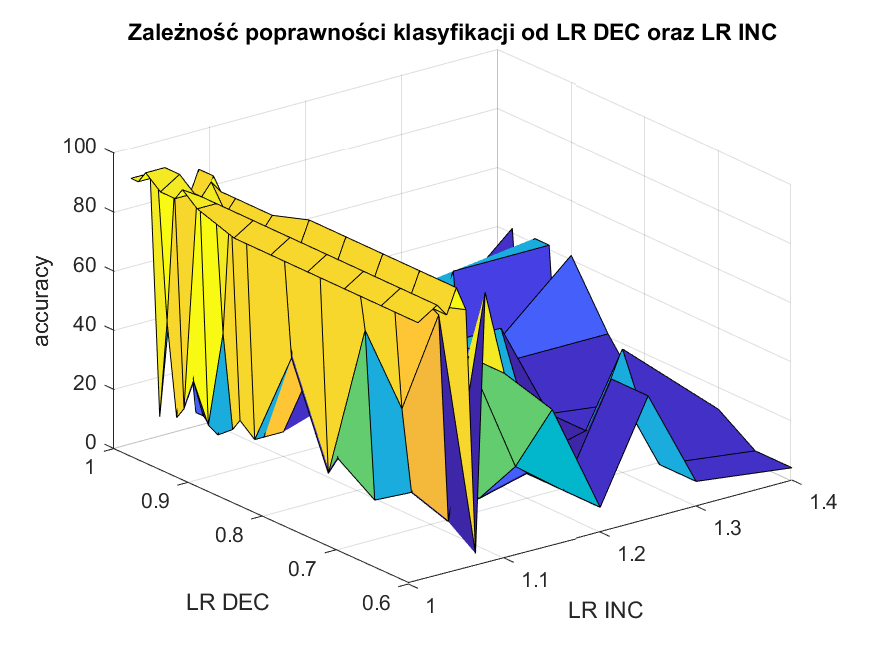
\includegraphics[width=16cm]{figures/Retarded_3.png}
	\caption{Poprawność klasyfikacji sieci uczonej osłabionym algorytmem przy er~=~1.07 S1~=~4 oraz S2~=~10}
	\label{Fig:Retarded3}
\end{figure}

Zauważalna była również wspomniana wcześniej różnica w czasie działania sieci.
W przypadku algorytmu klasycznego sieć zakończyła naukę przed dotarciem do granicznej iteracji w 168 na 169 przypadków testowych.
Średnia liczba iteracji (epok) wyniosła w tym przypadku  ok. 372 zaś średnia poprawność klasyfikacji - ok. 73\%
W przypadku algorytmu ograniczonego, sieć zakończyła naukę przed osiągnięciem granicznej epoki jedynie w 62 spośród 169 przypadków testowych.
Dysproporcja ta przełożyła się bezpośrednio na średnią liczbę epok, która wyniosła 6376 - blisko dwukrotność wartości osiągniętej przez algorytm klasyczny.
Duża liczba epok nie przełożyła się jednak na lepsze wyniki poprawności klasyfikacji.
Przy walidacji krzyżowej, sieć uczona osłabionym algorytmem osiągnęła śrendnio  jednie 43\% poprawności klasyfikacji, co potwierdza wysunięte na podstawie wykresów wnioski o gorszej efektywności takiego sposobu uczenia.

\clearpage
\addcontentsline{toc}{section}{Literatura}

\begin{thebibliography}{4}
	\bibitem{kiaMultiLayer} http://materialy.prz-rzeszow.pl/pracownik/pliki/34/sztuczna-inteligencja-cw9-siec-wielowarstw.pdf (Dostęp 05.06.2022r.)
	\bibitem{kiaSingleLayer} http://materialy.prz-rzeszow.pl/pracownik/pliki/34/sztuczna-inteligencja-cw8-siec-jednowarstw.pdf (Dostęp 05.06.2022r.)
	\bibitem{nndl} Nielsen M.: Neural Networks and Deep Learning. http://neuralnetworksanddeeplearning.com/ (Dostęp. 05.06.2022r.)
	\bibitem{kiaAcc} http://materialy.prz-rzeszow.pl/pracownik/pliki/34/sztuczna-inteligencja-cw10-przysp-uczenia.pdf (Dostęp 13.06.2022r.)
	\bibitem{nnd} Hagan T.M., Demuth H.B., Beale M.H.: Neural Network Design. https://hagan.okstate.edu/NNDesign.pdf (Dostęp 13.06.2022r.)
\end{thebibliography}

\clearpage


\end{document} 
